\documentclass[twoside]{book}

% Packages required by doxygen
\usepackage{fixltx2e}
\usepackage{calc}
\usepackage{doxygen}
\usepackage[export]{adjustbox} % also loads graphicx
\usepackage{graphicx}
\usepackage[utf8]{inputenc}
\usepackage{makeidx}
\usepackage{multicol}
\usepackage{multirow}
\PassOptionsToPackage{warn}{textcomp}
\usepackage{textcomp}
\usepackage[nointegrals]{wasysym}
\usepackage[table]{xcolor}

% Font selection
\usepackage[T1]{fontenc}
\usepackage[scaled=.90]{helvet}
\usepackage{courier}
\usepackage{amssymb}
\usepackage{sectsty}
\renewcommand{\familydefault}{\sfdefault}
\allsectionsfont{%
  \fontseries{bc}\selectfont%
  \color{darkgray}%
}
\renewcommand{\DoxyLabelFont}{%
  \fontseries{bc}\selectfont%
  \color{darkgray}%
}
\newcommand{\+}{\discretionary{\mbox{\scriptsize$\hookleftarrow$}}{}{}}

% Page & text layout
\usepackage{geometry}
\geometry{%
  a4paper,%
  top=2.5cm,%
  bottom=2.5cm,%
  left=2.5cm,%
  right=2.5cm%
}
\tolerance=750
\hfuzz=15pt
\hbadness=750
\setlength{\emergencystretch}{15pt}
\setlength{\parindent}{0cm}
\setlength{\parskip}{3ex plus 2ex minus 2ex}
\makeatletter
\renewcommand{\paragraph}{%
  \@startsection{paragraph}{4}{0ex}{-1.0ex}{1.0ex}{%
    \normalfont\normalsize\bfseries\SS@parafont%
  }%
}
\renewcommand{\subparagraph}{%
  \@startsection{subparagraph}{5}{0ex}{-1.0ex}{1.0ex}{%
    \normalfont\normalsize\bfseries\SS@subparafont%
  }%
}
\makeatother

% Headers & footers
\usepackage{fancyhdr}
\pagestyle{fancyplain}
\fancyhead[LE]{\fancyplain{}{\bfseries\thepage}}
\fancyhead[CE]{\fancyplain{}{}}
\fancyhead[RE]{\fancyplain{}{\bfseries\leftmark}}
\fancyhead[LO]{\fancyplain{}{\bfseries\rightmark}}
\fancyhead[CO]{\fancyplain{}{}}
\fancyhead[RO]{\fancyplain{}{\bfseries\thepage}}
\fancyfoot[LE]{\fancyplain{}{}}
\fancyfoot[CE]{\fancyplain{}{}}
\fancyfoot[RE]{\fancyplain{}{\bfseries\scriptsize Generated by Doxygen }}
\fancyfoot[LO]{\fancyplain{}{\bfseries\scriptsize Generated by Doxygen }}
\fancyfoot[CO]{\fancyplain{}{}}
\fancyfoot[RO]{\fancyplain{}{}}
\renewcommand{\footrulewidth}{0.4pt}
\renewcommand{\chaptermark}[1]{%
  \markboth{#1}{}%
}
\renewcommand{\sectionmark}[1]{%
  \markright{\thesection\ #1}%
}

% Indices & bibliography
\usepackage{natbib}
\usepackage[titles]{tocloft}
\setcounter{tocdepth}{3}
\setcounter{secnumdepth}{5}
\makeindex

% Hyperlinks (required, but should be loaded last)
\usepackage{ifpdf}
\ifpdf
  \usepackage[pdftex,pagebackref=true]{hyperref}
\else
  \usepackage[ps2pdf,pagebackref=true]{hyperref}
\fi
\hypersetup{%
  colorlinks=true,%
  linkcolor=blue,%
  citecolor=blue,%
  unicode%
}

% Custom commands
\newcommand{\clearemptydoublepage}{%
  \newpage{\pagestyle{empty}\cleardoublepage}%
}

\usepackage{caption}
\captionsetup{labelsep=space,justification=centering,font={bf},singlelinecheck=off,skip=4pt,position=top}

%===== C O N T E N T S =====

\begin{document}

% Titlepage & ToC
\hypersetup{pageanchor=false,
             bookmarksnumbered=true,
             pdfencoding=unicode
            }
\pagenumbering{roman}
\begin{titlepage}
\vspace*{7cm}
\begin{center}%
{\Large Project-\/1 Donald }\\
\vspace*{1cm}
{\large Generated by Doxygen 1.8.11}\\
\end{center}
\end{titlepage}
\clearemptydoublepage
\tableofcontents
\clearemptydoublepage
\pagenumbering{arabic}
\hypersetup{pageanchor=true}

%--- Begin generated contents ---
\chapter{Hierarchical Index}
\section{Class Hierarchy}
This inheritance list is sorted roughly, but not completely, alphabetically\+:\begin{DoxyCompactList}
\item \contentsline{section}{Actor}{\pageref{classActor}}{}
\begin{DoxyCompactList}
\item \contentsline{section}{Centipede}{\pageref{classCentipede}}{}
\item \contentsline{section}{Hero}{\pageref{classHero}}{}
\begin{DoxyCompactList}
\item \contentsline{section}{Reporter}{\pageref{classReporter}}{}
\item \contentsline{section}{S\+JW}{\pageref{classSJW}}{}
\end{DoxyCompactList}
\item \contentsline{section}{Miss\+Universe}{\pageref{classMissUniverse}}{}
\item \contentsline{section}{Politician}{\pageref{classPolitician}}{}
\item \contentsline{section}{The\+Donald}{\pageref{classTheDonald}}{}
\end{DoxyCompactList}
\item \contentsline{section}{Floor$<$ T $>$}{\pageref{classFloor}}{}
\item \contentsline{section}{Floor$<$ Actor $\ast$ $>$}{\pageref{classFloor}}{}
\item \contentsline{section}{R\+NG}{\pageref{classRNG}}{}
\item runtime\+\_\+error\begin{DoxyCompactList}
\item \contentsline{section}{T\+T\+Exception}{\pageref{classTTException}}{}
\end{DoxyCompactList}
\item \contentsline{section}{Trump\+Tower}{\pageref{classTrumpTower}}{}
\end{DoxyCompactList}

\chapter{Class Index}
\section{Class List}
Here are the classes, structs, unions and interfaces with brief descriptions\+:\begin{DoxyCompactList}
\item\contentsline{section}{\hyperlink{classActor}{Actor} }{\pageref{classActor}}{}
\item\contentsline{section}{\hyperlink{classCentipede}{Centipede} }{\pageref{classCentipede}}{}
\item\contentsline{section}{\hyperlink{classFloor}{Floor$<$ T $>$} }{\pageref{classFloor}}{}
\item\contentsline{section}{\hyperlink{classHero}{Hero} }{\pageref{classHero}}{}
\item\contentsline{section}{\hyperlink{classMissUniverse}{Miss\+Universe} }{\pageref{classMissUniverse}}{}
\item\contentsline{section}{\hyperlink{classPolitician}{Politician} }{\pageref{classPolitician}}{}
\item\contentsline{section}{\hyperlink{classReporter}{Reporter} }{\pageref{classReporter}}{}
\item\contentsline{section}{\hyperlink{classRNG}{R\+NG} }{\pageref{classRNG}}{}
\item\contentsline{section}{\hyperlink{classSJW}{S\+JW} }{\pageref{classSJW}}{}
\item\contentsline{section}{\hyperlink{classTheDonald}{The\+Donald} }{\pageref{classTheDonald}}{}
\item\contentsline{section}{\hyperlink{classTrumpTower}{Trump\+Tower} }{\pageref{classTrumpTower}}{}
\item\contentsline{section}{\hyperlink{classTTException}{T\+T\+Exception} }{\pageref{classTTException}}{}
\end{DoxyCompactList}

\chapter{File Index}
\section{File List}
Here is a list of all files with brief descriptions\+:\begin{DoxyCompactList}
\item\contentsline{section}{src/\hyperlink{actor_8cpp}{actor.\+cpp} }{\pageref{actor_8cpp}}{}
\item\contentsline{section}{src/\hyperlink{actor_8h}{actor.\+h} }{\pageref{actor_8h}}{}
\item\contentsline{section}{src/\hyperlink{centipede_8cpp}{centipede.\+cpp} }{\pageref{centipede_8cpp}}{}
\item\contentsline{section}{src/\hyperlink{centipede_8h}{centipede.\+h} }{\pageref{centipede_8h}}{}
\item\contentsline{section}{src/\hyperlink{direction_8h}{direction.\+h} }{\pageref{direction_8h}}{}
\item\contentsline{section}{src/\hyperlink{floor_8cpp}{floor.\+cpp} }{\pageref{floor_8cpp}}{}
\item\contentsline{section}{src/\hyperlink{floor_8h}{floor.\+h} }{\pageref{floor_8h}}{}
\item\contentsline{section}{src/\hyperlink{hero_8cpp}{hero.\+cpp} }{\pageref{hero_8cpp}}{}
\item\contentsline{section}{src/\hyperlink{hero_8h}{hero.\+h} }{\pageref{hero_8h}}{}
\item\contentsline{section}{src/\hyperlink{miss__universe_8cpp}{miss\+\_\+universe.\+cpp} }{\pageref{miss__universe_8cpp}}{}
\item\contentsline{section}{src/\hyperlink{miss__universe_8h}{miss\+\_\+universe.\+h} }{\pageref{miss__universe_8h}}{}
\item\contentsline{section}{src/\hyperlink{politician_8cpp}{politician.\+cpp} }{\pageref{politician_8cpp}}{}
\item\contentsline{section}{src/\hyperlink{politician_8h}{politician.\+h} }{\pageref{politician_8h}}{}
\item\contentsline{section}{src/\hyperlink{rand__test_8cpp}{rand\+\_\+test.\+cpp} }{\pageref{rand__test_8cpp}}{}
\item\contentsline{section}{src/\hyperlink{reporter_8cpp}{reporter.\+cpp} }{\pageref{reporter_8cpp}}{}
\item\contentsline{section}{src/\hyperlink{reporter_8h}{reporter.\+h} }{\pageref{reporter_8h}}{}
\item\contentsline{section}{src/\hyperlink{rng_8cpp}{rng.\+cpp} }{\pageref{rng_8cpp}}{}
\item\contentsline{section}{src/\hyperlink{rng_8h}{rng.\+h} }{\pageref{rng_8h}}{}
\item\contentsline{section}{src/\hyperlink{sjw_8cpp}{sjw.\+cpp} }{\pageref{sjw_8cpp}}{}
\item\contentsline{section}{src/\hyperlink{sjw_8h}{sjw.\+h} }{\pageref{sjw_8h}}{}
\item\contentsline{section}{src/\hyperlink{the__donald_8cpp}{the\+\_\+donald.\+cpp} }{\pageref{the__donald_8cpp}}{}
\item\contentsline{section}{src/\hyperlink{the__donald_8h}{the\+\_\+donald.\+h} }{\pageref{the__donald_8h}}{}
\item\contentsline{section}{src/\hyperlink{trump__tower_8cpp}{trump\+\_\+tower.\+cpp} }{\pageref{trump__tower_8cpp}}{}
\item\contentsline{section}{src/\hyperlink{trump__tower_8h}{trump\+\_\+tower.\+h} }{\pageref{trump__tower_8h}}{}
\item\contentsline{section}{src/\hyperlink{tt__exception_8h}{tt\+\_\+exception.\+h} }{\pageref{tt__exception_8h}}{}
\item\contentsline{section}{src/\hyperlink{tt__main_8cpp}{tt\+\_\+main.\+cpp} }{\pageref{tt__main_8cpp}}{}
\end{DoxyCompactList}

\chapter{Class Documentation}
\hypertarget{classActor}{}\section{Actor Class Reference}
\label{classActor}\index{Actor@{Actor}}


{\ttfamily \#include $<$actor.\+h$>$}



Inheritance diagram for Actor\+:
\nopagebreak
\begin{figure}[H]
\begin{center}
\leavevmode
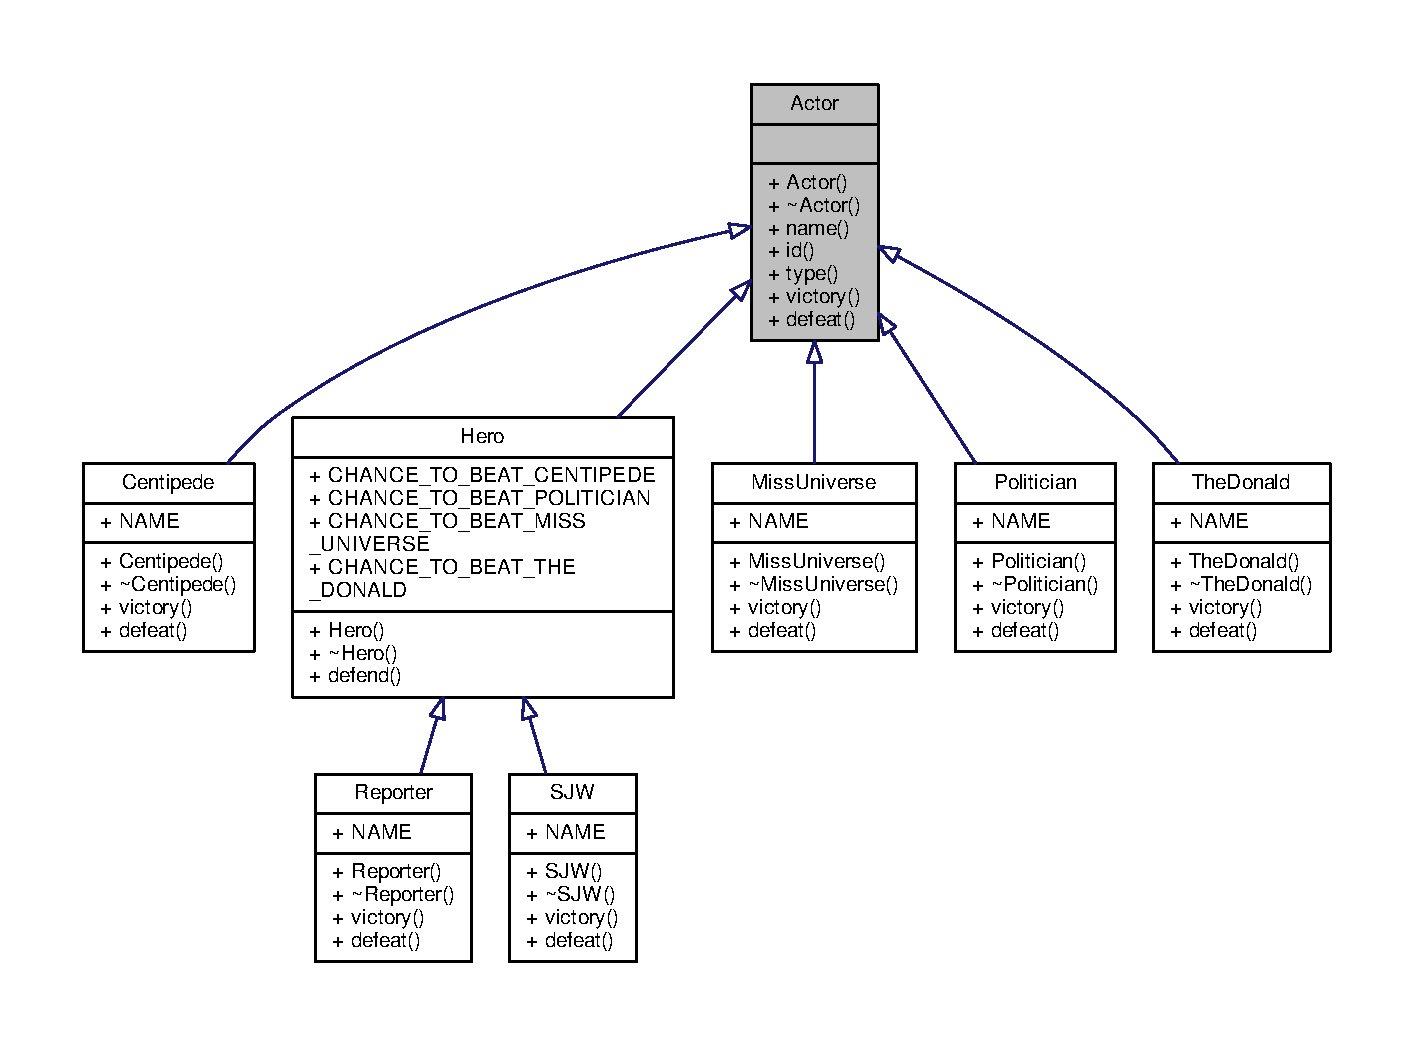
\includegraphics[width=350pt]{classActor__inherit__graph}
\end{center}
\end{figure}


Collaboration diagram for Actor\+:
\nopagebreak
\begin{figure}[H]
\begin{center}
\leavevmode
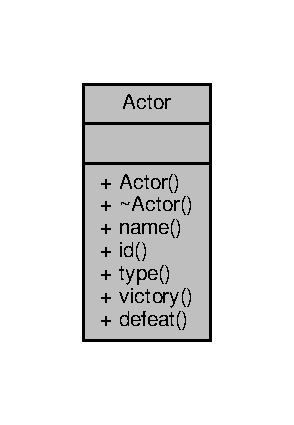
\includegraphics[width=141pt]{classActor__coll__graph}
\end{center}
\end{figure}
\subsection*{Public Types}
\begin{DoxyCompactItemize}
\item 
enum \hyperlink{classActor_a398752837eee9970ca00a3565e52c4da}{Actor\+Type} \{ \\*
\hyperlink{classActor_a398752837eee9970ca00a3565e52c4daaca4c443e9d37143364c2760158033d08}{C\+E\+N\+T\+I\+P\+E\+DE}, 
\hyperlink{classActor_a398752837eee9970ca00a3565e52c4daacf7f8a23b2a3995ab6777cb142cec6dc}{M\+I\+S\+S\+\_\+\+U\+N\+I\+V\+E\+R\+SE}, 
\hyperlink{classActor_a398752837eee9970ca00a3565e52c4daa7c3965a675a848e7e3d0c28a9218e20a}{P\+O\+L\+I\+T\+I\+C\+I\+AN}, 
\hyperlink{classActor_a398752837eee9970ca00a3565e52c4daa2911d77bb4a8255879b4684d6a84668d}{R\+E\+P\+O\+R\+T\+ER}, 
\\*
\hyperlink{classActor_a398752837eee9970ca00a3565e52c4daa6f51cf00ba9bc370ee69e35b1fb2c8aa}{S\+O\+C\+I\+A\+L\+\_\+\+J\+U\+S\+T\+I\+C\+E\+\_\+\+W\+A\+R\+R\+I\+OR}, 
\hyperlink{classActor_a398752837eee9970ca00a3565e52c4daa487ebaaccf7772d5a8bfb16b2a4c8e3c}{T\+H\+E\+\_\+\+D\+O\+N\+A\+LD}
 \}
\end{DoxyCompactItemize}
\subsection*{Public Member Functions}
\begin{DoxyCompactItemize}
\item 
\hyperlink{classActor_abe57954a691a017c6ee051d6d21baf13}{Actor} (const std\+::string \&\hyperlink{classActor_a400c24cfb4609e95e869bfe970f386c5}{name}, unsigned int \hyperlink{classActor_a084438abd4bcb9d5e17b8ad75b0f5984}{id}, \hyperlink{classActor_a398752837eee9970ca00a3565e52c4da}{Actor\+Type} \hyperlink{classActor_a2be506fc6785b49d642a1b8f445c5c00}{type})
\item 
virtual \hyperlink{classActor_ad807fe8f85e72ab263a0c05e3231cb39}{$\sim$\+Actor} ()
\item 
std\+::string \hyperlink{classActor_a400c24cfb4609e95e869bfe970f386c5}{name} () const 
\item 
unsigned int \hyperlink{classActor_a084438abd4bcb9d5e17b8ad75b0f5984}{id} () const 
\item 
\hyperlink{classActor_a398752837eee9970ca00a3565e52c4da}{Actor\+Type} \hyperlink{classActor_a2be506fc6785b49d642a1b8f445c5c00}{type} () const 
\item 
virtual std\+::string \hyperlink{classActor_a1595ffb3d753120a9e74eac0bd69adf1}{victory} (const \hyperlink{classActor}{Actor} \&other) const =0
\item 
virtual std\+::string \hyperlink{classActor_a0405c30d4ad11809647d2bf4e78026a7}{defeat} (const \hyperlink{classActor}{Actor} \&other) const =0
\end{DoxyCompactItemize}


\subsection{Detailed Description}
Abstract \hyperlink{classActor}{Actor} class 

\subsection{Member Enumeration Documentation}
\index{Actor@{Actor}!Actor\+Type@{Actor\+Type}}
\index{Actor\+Type@{Actor\+Type}!Actor@{Actor}}
\subsubsection[{\texorpdfstring{Actor\+Type}{ActorType}}]{\setlength{\rightskip}{0pt plus 5cm}enum {\bf Actor\+::\+Actor\+Type}}\hypertarget{classActor_a398752837eee9970ca00a3565e52c4da}{}\label{classActor_a398752837eee9970ca00a3565e52c4da}
enum Actor\+Type represents 6 types of actors \+: C\+E\+N\+T\+I\+P\+E\+DE, M\+I\+S\+S\+\_\+\+U\+N\+I\+V\+E\+R\+SE, P\+O\+L\+I\+T\+I\+C\+I\+AN, R\+E\+P\+O\+R\+T\+ER, S\+O\+C\+I\+A\+L\+\_\+\+J\+U\+S\+T\+I\+C\+E\+\_\+\+W\+A\+R\+R\+I\+OR, T\+H\+E\+\_\+\+D\+O\+N\+A\+LD \begin{Desc}
\item[Enumerator]\par
\begin{description}
\index{C\+E\+N\+T\+I\+P\+E\+DE@{C\+E\+N\+T\+I\+P\+E\+DE}!Actor@{Actor}}\index{Actor@{Actor}!C\+E\+N\+T\+I\+P\+E\+DE@{C\+E\+N\+T\+I\+P\+E\+DE}}\item[{\em 
C\+E\+N\+T\+I\+P\+E\+DE\hypertarget{classActor_a398752837eee9970ca00a3565e52c4daaca4c443e9d37143364c2760158033d08}{}\label{classActor_a398752837eee9970ca00a3565e52c4daaca4c443e9d37143364c2760158033d08}
}]\index{M\+I\+S\+S\+\_\+\+U\+N\+I\+V\+E\+R\+SE@{M\+I\+S\+S\+\_\+\+U\+N\+I\+V\+E\+R\+SE}!Actor@{Actor}}\index{Actor@{Actor}!M\+I\+S\+S\+\_\+\+U\+N\+I\+V\+E\+R\+SE@{M\+I\+S\+S\+\_\+\+U\+N\+I\+V\+E\+R\+SE}}\item[{\em 
M\+I\+S\+S\+\_\+\+U\+N\+I\+V\+E\+R\+SE\hypertarget{classActor_a398752837eee9970ca00a3565e52c4daacf7f8a23b2a3995ab6777cb142cec6dc}{}\label{classActor_a398752837eee9970ca00a3565e52c4daacf7f8a23b2a3995ab6777cb142cec6dc}
}]\index{P\+O\+L\+I\+T\+I\+C\+I\+AN@{P\+O\+L\+I\+T\+I\+C\+I\+AN}!Actor@{Actor}}\index{Actor@{Actor}!P\+O\+L\+I\+T\+I\+C\+I\+AN@{P\+O\+L\+I\+T\+I\+C\+I\+AN}}\item[{\em 
P\+O\+L\+I\+T\+I\+C\+I\+AN\hypertarget{classActor_a398752837eee9970ca00a3565e52c4daa7c3965a675a848e7e3d0c28a9218e20a}{}\label{classActor_a398752837eee9970ca00a3565e52c4daa7c3965a675a848e7e3d0c28a9218e20a}
}]\index{R\+E\+P\+O\+R\+T\+ER@{R\+E\+P\+O\+R\+T\+ER}!Actor@{Actor}}\index{Actor@{Actor}!R\+E\+P\+O\+R\+T\+ER@{R\+E\+P\+O\+R\+T\+ER}}\item[{\em 
R\+E\+P\+O\+R\+T\+ER\hypertarget{classActor_a398752837eee9970ca00a3565e52c4daa2911d77bb4a8255879b4684d6a84668d}{}\label{classActor_a398752837eee9970ca00a3565e52c4daa2911d77bb4a8255879b4684d6a84668d}
}]\index{S\+O\+C\+I\+A\+L\+\_\+\+J\+U\+S\+T\+I\+C\+E\+\_\+\+W\+A\+R\+R\+I\+OR@{S\+O\+C\+I\+A\+L\+\_\+\+J\+U\+S\+T\+I\+C\+E\+\_\+\+W\+A\+R\+R\+I\+OR}!Actor@{Actor}}\index{Actor@{Actor}!S\+O\+C\+I\+A\+L\+\_\+\+J\+U\+S\+T\+I\+C\+E\+\_\+\+W\+A\+R\+R\+I\+OR@{S\+O\+C\+I\+A\+L\+\_\+\+J\+U\+S\+T\+I\+C\+E\+\_\+\+W\+A\+R\+R\+I\+OR}}\item[{\em 
S\+O\+C\+I\+A\+L\+\_\+\+J\+U\+S\+T\+I\+C\+E\+\_\+\+W\+A\+R\+R\+I\+OR\hypertarget{classActor_a398752837eee9970ca00a3565e52c4daa6f51cf00ba9bc370ee69e35b1fb2c8aa}{}\label{classActor_a398752837eee9970ca00a3565e52c4daa6f51cf00ba9bc370ee69e35b1fb2c8aa}
}]\index{T\+H\+E\+\_\+\+D\+O\+N\+A\+LD@{T\+H\+E\+\_\+\+D\+O\+N\+A\+LD}!Actor@{Actor}}\index{Actor@{Actor}!T\+H\+E\+\_\+\+D\+O\+N\+A\+LD@{T\+H\+E\+\_\+\+D\+O\+N\+A\+LD}}\item[{\em 
T\+H\+E\+\_\+\+D\+O\+N\+A\+LD\hypertarget{classActor_a398752837eee9970ca00a3565e52c4daa487ebaaccf7772d5a8bfb16b2a4c8e3c}{}\label{classActor_a398752837eee9970ca00a3565e52c4daa487ebaaccf7772d5a8bfb16b2a4c8e3c}
}]\end{description}
\end{Desc}


\subsection{Constructor \& Destructor Documentation}
\index{Actor@{Actor}!Actor@{Actor}}
\index{Actor@{Actor}!Actor@{Actor}}
\subsubsection[{\texorpdfstring{Actor(const std\+::string \&name, unsigned int id, Actor\+Type type)}{Actor(const std::string &name, unsigned int id, ActorType type)}}]{\setlength{\rightskip}{0pt plus 5cm}Actor\+::\+Actor (
\begin{DoxyParamCaption}
\item[{const std\+::string \&}]{name, }
\item[{unsigned int}]{id, }
\item[{{\bf Actor\+Type}}]{type}
\end{DoxyParamCaption}
)}\hypertarget{classActor_abe57954a691a017c6ee051d6d21baf13}{}\label{classActor_abe57954a691a017c6ee051d6d21baf13}
Creating new actor


\begin{DoxyParams}{Parameters}
{\em name} & name of the actor \\
\hline
{\em id} & unqiue id of the actor \\
\hline
{\em type} & type of the actor \\
\hline
\end{DoxyParams}
\index{Actor@{Actor}!````~Actor@{$\sim$\+Actor}}
\index{````~Actor@{$\sim$\+Actor}!Actor@{Actor}}
\subsubsection[{\texorpdfstring{$\sim$\+Actor()}{~Actor()}}]{\setlength{\rightskip}{0pt plus 5cm}Actor\+::$\sim$\+Actor (
\begin{DoxyParamCaption}
{}
\end{DoxyParamCaption}
)\hspace{0.3cm}{\ttfamily [virtual]}}\hypertarget{classActor_ad807fe8f85e72ab263a0c05e3231cb39}{}\label{classActor_ad807fe8f85e72ab263a0c05e3231cb39}
Destructor for actor 

\subsection{Member Function Documentation}
\index{Actor@{Actor}!defeat@{defeat}}
\index{defeat@{defeat}!Actor@{Actor}}
\subsubsection[{\texorpdfstring{defeat(const Actor \&other) const =0}{defeat(const Actor &other) const =0}}]{\setlength{\rightskip}{0pt plus 5cm}virtual std\+::string Actor\+::defeat (
\begin{DoxyParamCaption}
\item[{const {\bf Actor} \&}]{other}
\end{DoxyParamCaption}
) const\hspace{0.3cm}{\ttfamily [pure virtual]}}\hypertarget{classActor_a0405c30d4ad11809647d2bf4e78026a7}{}\label{classActor_a0405c30d4ad11809647d2bf4e78026a7}


Implemented in \hyperlink{classSJW_a04d480d0bedb684591a1a14d41b93257}{S\+JW}, \hyperlink{classMissUniverse_af8842e3ec345796fcdadca07a79442b0}{Miss\+Universe}, \hyperlink{classReporter_a6147cf4ee48d5c81e72538d39c79d228}{Reporter}, \hyperlink{classTheDonald_ac6920f6026c3b0d91afbce90f6f07fad}{The\+Donald}, \hyperlink{classPolitician_a0734a1c1deed35b36b02f83b2c9ee46c}{Politician}, and \hyperlink{classCentipede_ae7cf6ce3b3b3ce66fe82986fd31d7be0}{Centipede}.

\index{Actor@{Actor}!id@{id}}
\index{id@{id}!Actor@{Actor}}
\subsubsection[{\texorpdfstring{id() const }{id() const }}]{\setlength{\rightskip}{0pt plus 5cm}unsigned int Actor\+::id (
\begin{DoxyParamCaption}
{}
\end{DoxyParamCaption}
) const}\hypertarget{classActor_a084438abd4bcb9d5e17b8ad75b0f5984}{}\label{classActor_a084438abd4bcb9d5e17b8ad75b0f5984}
get the id of the actor

\begin{DoxyReturn}{Returns}
id of actor 
\end{DoxyReturn}
\index{Actor@{Actor}!name@{name}}
\index{name@{name}!Actor@{Actor}}
\subsubsection[{\texorpdfstring{name() const }{name() const }}]{\setlength{\rightskip}{0pt plus 5cm}std\+::string Actor\+::name (
\begin{DoxyParamCaption}
{}
\end{DoxyParamCaption}
) const}\hypertarget{classActor_a400c24cfb4609e95e869bfe970f386c5}{}\label{classActor_a400c24cfb4609e95e869bfe970f386c5}
get the name of the actor

\begin{DoxyReturn}{Returns}
actor\textquotesingle{}s name 
\end{DoxyReturn}
\index{Actor@{Actor}!type@{type}}
\index{type@{type}!Actor@{Actor}}
\subsubsection[{\texorpdfstring{type() const }{type() const }}]{\setlength{\rightskip}{0pt plus 5cm}{\bf Actor\+::\+Actor\+Type} Actor\+::type (
\begin{DoxyParamCaption}
{}
\end{DoxyParamCaption}
) const}\hypertarget{classActor_a2be506fc6785b49d642a1b8f445c5c00}{}\label{classActor_a2be506fc6785b49d642a1b8f445c5c00}
get the type of actor

\begin{DoxyReturn}{Returns}
actor type 
\end{DoxyReturn}
\index{Actor@{Actor}!victory@{victory}}
\index{victory@{victory}!Actor@{Actor}}
\subsubsection[{\texorpdfstring{victory(const Actor \&other) const =0}{victory(const Actor &other) const =0}}]{\setlength{\rightskip}{0pt plus 5cm}virtual std\+::string Actor\+::victory (
\begin{DoxyParamCaption}
\item[{const {\bf Actor} \&}]{other}
\end{DoxyParamCaption}
) const\hspace{0.3cm}{\ttfamily [pure virtual]}}\hypertarget{classActor_a1595ffb3d753120a9e74eac0bd69adf1}{}\label{classActor_a1595ffb3d753120a9e74eac0bd69adf1}

\begin{DoxyParams}{Parameters}
{\em other} & \\
\hline
\end{DoxyParams}
\begin{DoxyReturn}{Returns}

\end{DoxyReturn}


Implemented in \hyperlink{classSJW_af9bffa85da9c04559f38210f11a80c1d}{S\+JW}, \hyperlink{classMissUniverse_aac659076d954d5342ba494a993eab2fd}{Miss\+Universe}, \hyperlink{classReporter_ac0c496d5f8f3f56c71d2afe6ab53490e}{Reporter}, \hyperlink{classTheDonald_abee1d5bb4910c657ffd41fc745298cdc}{The\+Donald}, \hyperlink{classPolitician_a7428489cb0380195cc5d74faeece6355}{Politician}, and \hyperlink{classCentipede_a1b995576767d3eff9bfcac599ec35ddf}{Centipede}.



The documentation for this class was generated from the following files\+:\begin{DoxyCompactItemize}
\item 
src/\hyperlink{actor_8h}{actor.\+h}\item 
src/\hyperlink{actor_8cpp}{actor.\+cpp}\end{DoxyCompactItemize}

\hypertarget{classCentipede}{}\section{Centipede Class Reference}
\label{classCentipede}\index{Centipede@{Centipede}}


{\ttfamily \#include $<$centipede.\+h$>$}



Inheritance diagram for Centipede\+:
\nopagebreak
\begin{figure}[H]
\begin{center}
\leavevmode
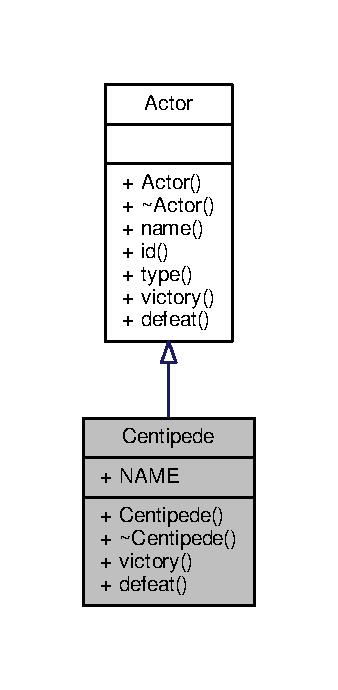
\includegraphics[width=162pt]{classCentipede__inherit__graph}
\end{center}
\end{figure}


Collaboration diagram for Centipede\+:
\nopagebreak
\begin{figure}[H]
\begin{center}
\leavevmode
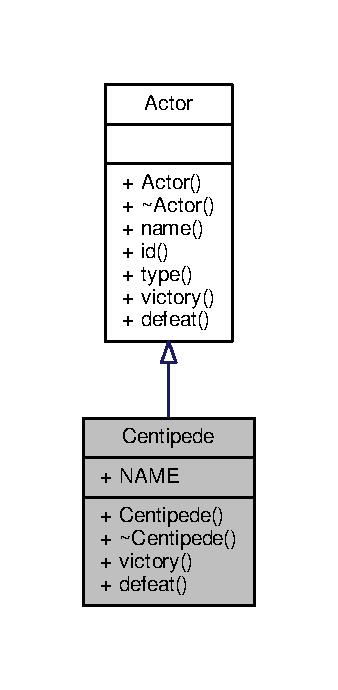
\includegraphics[width=162pt]{classCentipede__coll__graph}
\end{center}
\end{figure}
\subsection*{Public Member Functions}
\begin{DoxyCompactItemize}
\item 
\hyperlink{classCentipede_ae0fed98579ba2b20049697c97de32cfb}{Centipede} (unsigned int \hyperlink{classActor_a084438abd4bcb9d5e17b8ad75b0f5984}{id})
\item 
\hyperlink{classCentipede_a960454b63733792b46ab91c959e8ec2c}{$\sim$\+Centipede} ()
\item 
virtual std\+::string \hyperlink{classCentipede_a1b995576767d3eff9bfcac599ec35ddf}{victory} (const \hyperlink{classActor}{Actor} \&other) const 
\item 
virtual std\+::string \hyperlink{classCentipede_ae7cf6ce3b3b3ce66fe82986fd31d7be0}{defeat} (const \hyperlink{classActor}{Actor} \&other) const 
\end{DoxyCompactItemize}
\subsection*{Static Public Attributes}
\begin{DoxyCompactItemize}
\item 
static const std\+::string \hyperlink{classCentipede_a9eb91c34048cb51599b5c3bcac6dfa64}{N\+A\+ME} = \char`\"{}Centipede\char`\"{}
\end{DoxyCompactItemize}
\subsection*{Additional Inherited Members}


\subsection{Constructor \& Destructor Documentation}
\index{Centipede@{Centipede}!Centipede@{Centipede}}
\index{Centipede@{Centipede}!Centipede@{Centipede}}
\subsubsection[{\texorpdfstring{Centipede(unsigned int id)}{Centipede(unsigned int id)}}]{\setlength{\rightskip}{0pt plus 5cm}Centipede\+::\+Centipede (
\begin{DoxyParamCaption}
\item[{unsigned int}]{id}
\end{DoxyParamCaption}
)}\hypertarget{classCentipede_ae0fed98579ba2b20049697c97de32cfb}{}\label{classCentipede_ae0fed98579ba2b20049697c97de32cfb}
\index{Centipede@{Centipede}!````~Centipede@{$\sim$\+Centipede}}
\index{````~Centipede@{$\sim$\+Centipede}!Centipede@{Centipede}}
\subsubsection[{\texorpdfstring{$\sim$\+Centipede()}{~Centipede()}}]{\setlength{\rightskip}{0pt plus 5cm}Centipede\+::$\sim$\+Centipede (
\begin{DoxyParamCaption}
{}
\end{DoxyParamCaption}
)}\hypertarget{classCentipede_a960454b63733792b46ab91c959e8ec2c}{}\label{classCentipede_a960454b63733792b46ab91c959e8ec2c}


\subsection{Member Function Documentation}
\index{Centipede@{Centipede}!defeat@{defeat}}
\index{defeat@{defeat}!Centipede@{Centipede}}
\subsubsection[{\texorpdfstring{defeat(const Actor \&other) const }{defeat(const Actor &other) const }}]{\setlength{\rightskip}{0pt plus 5cm}std\+::string Centipede\+::defeat (
\begin{DoxyParamCaption}
\item[{const {\bf Actor} \&}]{other}
\end{DoxyParamCaption}
) const\hspace{0.3cm}{\ttfamily [virtual]}}\hypertarget{classCentipede_ae7cf6ce3b3b3ce66fe82986fd31d7be0}{}\label{classCentipede_ae7cf6ce3b3b3ce66fe82986fd31d7be0}


Implements \hyperlink{classActor_a0405c30d4ad11809647d2bf4e78026a7}{Actor}.

\index{Centipede@{Centipede}!victory@{victory}}
\index{victory@{victory}!Centipede@{Centipede}}
\subsubsection[{\texorpdfstring{victory(const Actor \&other) const }{victory(const Actor &other) const }}]{\setlength{\rightskip}{0pt plus 5cm}std\+::string Centipede\+::victory (
\begin{DoxyParamCaption}
\item[{const {\bf Actor} \&}]{other}
\end{DoxyParamCaption}
) const\hspace{0.3cm}{\ttfamily [virtual]}}\hypertarget{classCentipede_a1b995576767d3eff9bfcac599ec35ddf}{}\label{classCentipede_a1b995576767d3eff9bfcac599ec35ddf}

\begin{DoxyParams}{Parameters}
{\em other} & \\
\hline
\end{DoxyParams}
\begin{DoxyReturn}{Returns}

\end{DoxyReturn}


Implements \hyperlink{classActor_a1595ffb3d753120a9e74eac0bd69adf1}{Actor}.



\subsection{Member Data Documentation}
\index{Centipede@{Centipede}!N\+A\+ME@{N\+A\+ME}}
\index{N\+A\+ME@{N\+A\+ME}!Centipede@{Centipede}}
\subsubsection[{\texorpdfstring{N\+A\+ME}{NAME}}]{\setlength{\rightskip}{0pt plus 5cm}const std\+::string Centipede\+::\+N\+A\+ME = \char`\"{}Centipede\char`\"{}\hspace{0.3cm}{\ttfamily [static]}}\hypertarget{classCentipede_a9eb91c34048cb51599b5c3bcac6dfa64}{}\label{classCentipede_a9eb91c34048cb51599b5c3bcac6dfa64}


The documentation for this class was generated from the following files\+:\begin{DoxyCompactItemize}
\item 
src/\hyperlink{centipede_8h}{centipede.\+h}\item 
src/\hyperlink{centipede_8cpp}{centipede.\+cpp}\end{DoxyCompactItemize}

\hypertarget{classFloor}{}\section{Floor$<$ T $>$ Class Template Reference}
\label{classFloor}\index{Floor$<$ T $>$@{Floor$<$ T $>$}}


{\ttfamily \#include $<$floor.\+h$>$}



Collaboration diagram for Floor$<$ T $>$\+:
\nopagebreak
\begin{figure}[H]
\begin{center}
\leavevmode
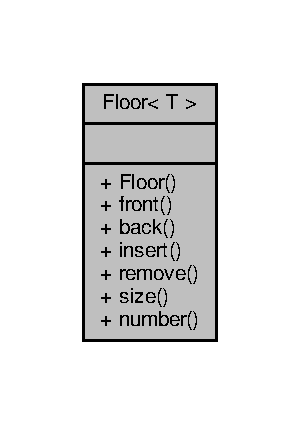
\includegraphics[width=144pt]{classFloor__coll__graph}
\end{center}
\end{figure}
\subsection*{Public Member Functions}
\begin{DoxyCompactItemize}
\item 
\hyperlink{classFloor_a3a53ede7923b19d33787663dfce4d7ca}{Floor} (unsigned int \hyperlink{classFloor_a30de5259aa79b701c36897502b9b6295}{number})
\item 
const T \& \hyperlink{classFloor_aff584554fded633dc29a87a96f7840a7}{front} (\hyperlink{direction_8h_a224b9163917ac32fc95a60d8c1eec3aa}{Direction} dir) const   throw (\+T\+T\+Exception)
\item 
const T \& \hyperlink{classFloor_a641151d981cdb1e27e82980f255d72d3}{back} (\hyperlink{direction_8h_a224b9163917ac32fc95a60d8c1eec3aa}{Direction} dir) const   throw (\+T\+T\+Exception)
\item 
void \hyperlink{classFloor_aae2be662bce4dc3ca0c18e029d85d628}{insert} (const T \&element, \hyperlink{direction_8h_a224b9163917ac32fc95a60d8c1eec3aa}{Direction} dir)
\item 
void \hyperlink{classFloor_a728395aeeae56e45da8cb9b13066aed5}{remove} (\hyperlink{direction_8h_a224b9163917ac32fc95a60d8c1eec3aa}{Direction} dir)  throw (\+T\+T\+Exception)
\item 
unsigned long \hyperlink{classFloor_a271b299427f7d246cb055b4012cf173d}{size} (\hyperlink{direction_8h_a224b9163917ac32fc95a60d8c1eec3aa}{Direction} dir) const 
\item 
unsigned int \hyperlink{classFloor_a30de5259aa79b701c36897502b9b6295}{number} () const 
\end{DoxyCompactItemize}


\subsection{Constructor \& Destructor Documentation}
\index{Floor@{Floor}!Floor@{Floor}}
\index{Floor@{Floor}!Floor@{Floor}}
\subsubsection[{\texorpdfstring{Floor(unsigned int number)}{Floor(unsigned int number)}}]{\setlength{\rightskip}{0pt plus 5cm}template$<$typename T $>$ {\bf Floor}$<$ T $>$\+::{\bf Floor} (
\begin{DoxyParamCaption}
\item[{unsigned int}]{number}
\end{DoxyParamCaption}
)}\hypertarget{classFloor_a3a53ede7923b19d33787663dfce4d7ca}{}\label{classFloor_a3a53ede7923b19d33787663dfce4d7ca}


\subsection{Member Function Documentation}
\index{Floor@{Floor}!back@{back}}
\index{back@{back}!Floor@{Floor}}
\subsubsection[{\texorpdfstring{back(\+Direction dir) const }{back(Direction dir) const }}]{\setlength{\rightskip}{0pt plus 5cm}template$<$typename T $>$ const T \& {\bf Floor}$<$ T $>$\+::back (
\begin{DoxyParamCaption}
\item[{{\bf Direction}}]{dir}
\end{DoxyParamCaption}
) const throw  {\bf T\+T\+Exception}) }\hypertarget{classFloor_a641151d981cdb1e27e82980f255d72d3}{}\label{classFloor_a641151d981cdb1e27e82980f255d72d3}
\index{Floor@{Floor}!front@{front}}
\index{front@{front}!Floor@{Floor}}
\subsubsection[{\texorpdfstring{front(\+Direction dir) const }{front(Direction dir) const }}]{\setlength{\rightskip}{0pt plus 5cm}template$<$typename T $>$ const T \& {\bf Floor}$<$ T $>$\+::front (
\begin{DoxyParamCaption}
\item[{{\bf Direction}}]{dir}
\end{DoxyParamCaption}
) const throw  {\bf T\+T\+Exception}) }\hypertarget{classFloor_aff584554fded633dc29a87a96f7840a7}{}\label{classFloor_aff584554fded633dc29a87a96f7840a7}
\index{Floor@{Floor}!insert@{insert}}
\index{insert@{insert}!Floor@{Floor}}
\subsubsection[{\texorpdfstring{insert(const T \&element, Direction dir)}{insert(const T &element, Direction dir)}}]{\setlength{\rightskip}{0pt plus 5cm}template$<$typename T$>$ void {\bf Floor}$<$ T $>$\+::insert (
\begin{DoxyParamCaption}
\item[{const T \&}]{element, }
\item[{{\bf Direction}}]{dir}
\end{DoxyParamCaption}
)}\hypertarget{classFloor_aae2be662bce4dc3ca0c18e029d85d628}{}\label{classFloor_aae2be662bce4dc3ca0c18e029d85d628}
\index{Floor@{Floor}!number@{number}}
\index{number@{number}!Floor@{Floor}}
\subsubsection[{\texorpdfstring{number() const }{number() const }}]{\setlength{\rightskip}{0pt plus 5cm}template$<$typename T $>$ unsigned int {\bf Floor}$<$ T $>$\+::number (
\begin{DoxyParamCaption}
{}
\end{DoxyParamCaption}
) const}\hypertarget{classFloor_a30de5259aa79b701c36897502b9b6295}{}\label{classFloor_a30de5259aa79b701c36897502b9b6295}
\index{Floor@{Floor}!remove@{remove}}
\index{remove@{remove}!Floor@{Floor}}
\subsubsection[{\texorpdfstring{remove(\+Direction dir)}{remove(Direction dir)}}]{\setlength{\rightskip}{0pt plus 5cm}template$<$typename T $>$ void {\bf Floor}$<$ T $>$\+::remove (
\begin{DoxyParamCaption}
\item[{{\bf Direction}}]{dir}
\end{DoxyParamCaption}
) throw  {\bf T\+T\+Exception}) }\hypertarget{classFloor_a728395aeeae56e45da8cb9b13066aed5}{}\label{classFloor_a728395aeeae56e45da8cb9b13066aed5}
\index{Floor@{Floor}!size@{size}}
\index{size@{size}!Floor@{Floor}}
\subsubsection[{\texorpdfstring{size(\+Direction dir) const }{size(Direction dir) const }}]{\setlength{\rightskip}{0pt plus 5cm}template$<$typename T $>$ unsigned long {\bf Floor}$<$ T $>$\+::size (
\begin{DoxyParamCaption}
\item[{{\bf Direction}}]{dir}
\end{DoxyParamCaption}
) const}\hypertarget{classFloor_a271b299427f7d246cb055b4012cf173d}{}\label{classFloor_a271b299427f7d246cb055b4012cf173d}


The documentation for this class was generated from the following files\+:\begin{DoxyCompactItemize}
\item 
src/\hyperlink{floor_8h}{floor.\+h}\item 
src/\hyperlink{floor_8cpp}{floor.\+cpp}\end{DoxyCompactItemize}

\hypertarget{classHero}{}\section{Hero Class Reference}
\label{classHero}\index{Hero@{Hero}}


{\ttfamily \#include $<$hero.\+h$>$}



Inheritance diagram for Hero\+:
\nopagebreak
\begin{figure}[H]
\begin{center}
\leavevmode
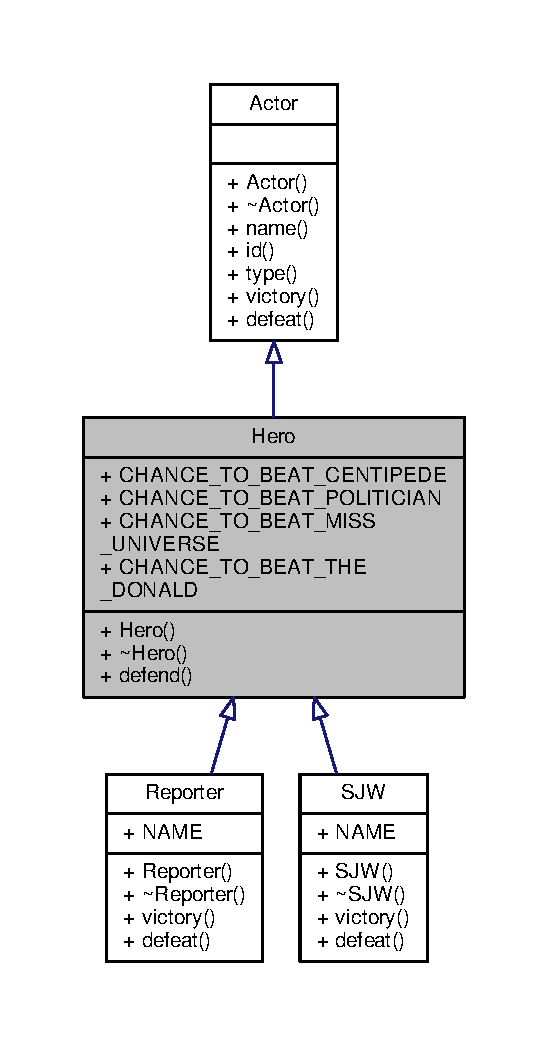
\includegraphics[width=263pt]{classHero__inherit__graph}
\end{center}
\end{figure}


Collaboration diagram for Hero\+:
\nopagebreak
\begin{figure}[H]
\begin{center}
\leavevmode
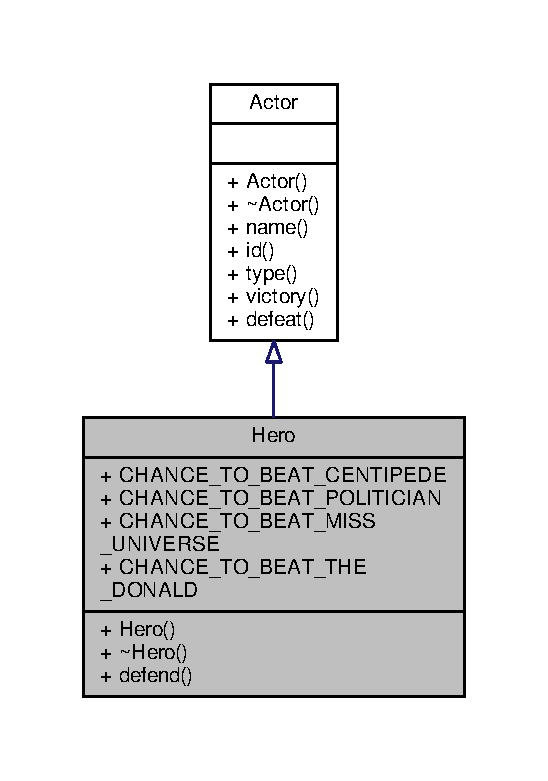
\includegraphics[width=263pt]{classHero__coll__graph}
\end{center}
\end{figure}
\subsection*{Public Member Functions}
\begin{DoxyCompactItemize}
\item 
\hyperlink{classHero_a29fa67296e31abaedeaedfdc39a9ed36}{Hero} (const std\+::string \&\hyperlink{classActor_a400c24cfb4609e95e869bfe970f386c5}{name}, unsigned int \hyperlink{classActor_a084438abd4bcb9d5e17b8ad75b0f5984}{id}, \hyperlink{classActor_a398752837eee9970ca00a3565e52c4da}{Actor\+::\+Actor\+Type} \hyperlink{classActor_a2be506fc6785b49d642a1b8f445c5c00}{type})
\item 
\hyperlink{classHero_a5aeef41ede5a80dc29c5acd7b553c4da}{$\sim$\+Hero} ()
\item 
bool \hyperlink{classHero_a7168d1fa26c3346cf0f541f4447bc05d}{defend} (const \hyperlink{classActor}{Actor} \&other) const 
\end{DoxyCompactItemize}
\subsection*{Static Public Attributes}
\begin{DoxyCompactItemize}
\item 
static const int \hyperlink{classHero_a79603131508da3c95d82594ff29ccb32}{C\+H\+A\+N\+C\+E\+\_\+\+T\+O\+\_\+\+B\+E\+A\+T\+\_\+\+C\+E\+N\+T\+I\+P\+E\+DE} = 90
\item 
static const int \hyperlink{classHero_a8fe3d6c05946b15de5b08e912fe226fc}{C\+H\+A\+N\+C\+E\+\_\+\+T\+O\+\_\+\+B\+E\+A\+T\+\_\+\+P\+O\+L\+I\+T\+I\+C\+I\+AN} = 80
\item 
static const int \hyperlink{classHero_a13075687fe82d8eee2bd7ef77222ca4f}{C\+H\+A\+N\+C\+E\+\_\+\+T\+O\+\_\+\+B\+E\+A\+T\+\_\+\+M\+I\+S\+S\+\_\+\+U\+N\+I\+V\+E\+R\+SE} = 70
\item 
static const int \hyperlink{classHero_a470885608dec7243532ca656b52feead}{C\+H\+A\+N\+C\+E\+\_\+\+T\+O\+\_\+\+B\+E\+A\+T\+\_\+\+T\+H\+E\+\_\+\+D\+O\+N\+A\+LD} = 25
\end{DoxyCompactItemize}
\subsection*{Additional Inherited Members}


\subsection{Detailed Description}
\hyperlink{classHero}{Hero} are basically Actors. hero\textquotesingle{}s can be either Social Justice warriors(\+S\+J\+W) or reporters. 

\subsection{Constructor \& Destructor Documentation}
\index{Hero@{Hero}!Hero@{Hero}}
\index{Hero@{Hero}!Hero@{Hero}}
\subsubsection[{\texorpdfstring{Hero(const std\+::string \&name, unsigned int id, Actor\+::\+Actor\+Type type)}{Hero(const std::string &name, unsigned int id, Actor::ActorType type)}}]{\setlength{\rightskip}{0pt plus 5cm}Hero\+::\+Hero (
\begin{DoxyParamCaption}
\item[{const std\+::string \&}]{name, }
\item[{unsigned int}]{id, }
\item[{{\bf Actor\+::\+Actor\+Type}}]{type}
\end{DoxyParamCaption}
)}\hypertarget{classHero_a29fa67296e31abaedeaedfdc39a9ed36}{}\label{classHero_a29fa67296e31abaedeaedfdc39a9ed36}
create new \hyperlink{classHero}{Hero} 
\begin{DoxyParams}{Parameters}
{\em name} & \+: \hyperlink{classHero}{Hero} name \\
\hline
{\em id} & \+: \hyperlink{classHero}{Hero} id \\
\hline
{\em type} & \+: \hyperlink{classHero}{Hero} type\+: \hyperlink{classSJW}{S\+JW} or \hyperlink{classReporter}{Reporter} \\
\hline
\end{DoxyParams}
\index{Hero@{Hero}!````~Hero@{$\sim$\+Hero}}
\index{````~Hero@{$\sim$\+Hero}!Hero@{Hero}}
\subsubsection[{\texorpdfstring{$\sim$\+Hero()}{~Hero()}}]{\setlength{\rightskip}{0pt plus 5cm}Hero\+::$\sim$\+Hero (
\begin{DoxyParamCaption}
{}
\end{DoxyParamCaption}
)}\hypertarget{classHero_a5aeef41ede5a80dc29c5acd7b553c4da}{}\label{classHero_a5aeef41ede5a80dc29c5acd7b553c4da}
Destroy the created \hyperlink{classHero}{Hero} 

\subsection{Member Function Documentation}
\index{Hero@{Hero}!defend@{defend}}
\index{defend@{defend}!Hero@{Hero}}
\subsubsection[{\texorpdfstring{defend(const Actor \&other) const }{defend(const Actor &other) const }}]{\setlength{\rightskip}{0pt plus 5cm}bool Hero\+::defend (
\begin{DoxyParamCaption}
\item[{const {\bf Actor} \&}]{other}
\end{DoxyParamCaption}
) const}\hypertarget{classHero_a7168d1fa26c3346cf0f541f4447bc05d}{}\label{classHero_a7168d1fa26c3346cf0f541f4447bc05d}
hero fights enemy 
\begin{DoxyParams}{Parameters}
{\em other} & \+: enemy \\
\hline
\end{DoxyParams}
\begin{DoxyReturn}{Returns}
true if hero else false 
\end{DoxyReturn}


\subsection{Member Data Documentation}
\index{Hero@{Hero}!C\+H\+A\+N\+C\+E\+\_\+\+T\+O\+\_\+\+B\+E\+A\+T\+\_\+\+C\+E\+N\+T\+I\+P\+E\+DE@{C\+H\+A\+N\+C\+E\+\_\+\+T\+O\+\_\+\+B\+E\+A\+T\+\_\+\+C\+E\+N\+T\+I\+P\+E\+DE}}
\index{C\+H\+A\+N\+C\+E\+\_\+\+T\+O\+\_\+\+B\+E\+A\+T\+\_\+\+C\+E\+N\+T\+I\+P\+E\+DE@{C\+H\+A\+N\+C\+E\+\_\+\+T\+O\+\_\+\+B\+E\+A\+T\+\_\+\+C\+E\+N\+T\+I\+P\+E\+DE}!Hero@{Hero}}
\subsubsection[{\texorpdfstring{C\+H\+A\+N\+C\+E\+\_\+\+T\+O\+\_\+\+B\+E\+A\+T\+\_\+\+C\+E\+N\+T\+I\+P\+E\+DE}{CHANCE_TO_BEAT_CENTIPEDE}}]{\setlength{\rightskip}{0pt plus 5cm}const int Hero\+::\+C\+H\+A\+N\+C\+E\+\_\+\+T\+O\+\_\+\+B\+E\+A\+T\+\_\+\+C\+E\+N\+T\+I\+P\+E\+DE = 90\hspace{0.3cm}{\ttfamily [static]}}\hypertarget{classHero_a79603131508da3c95d82594ff29ccb32}{}\label{classHero_a79603131508da3c95d82594ff29ccb32}
\index{Hero@{Hero}!C\+H\+A\+N\+C\+E\+\_\+\+T\+O\+\_\+\+B\+E\+A\+T\+\_\+\+M\+I\+S\+S\+\_\+\+U\+N\+I\+V\+E\+R\+SE@{C\+H\+A\+N\+C\+E\+\_\+\+T\+O\+\_\+\+B\+E\+A\+T\+\_\+\+M\+I\+S\+S\+\_\+\+U\+N\+I\+V\+E\+R\+SE}}
\index{C\+H\+A\+N\+C\+E\+\_\+\+T\+O\+\_\+\+B\+E\+A\+T\+\_\+\+M\+I\+S\+S\+\_\+\+U\+N\+I\+V\+E\+R\+SE@{C\+H\+A\+N\+C\+E\+\_\+\+T\+O\+\_\+\+B\+E\+A\+T\+\_\+\+M\+I\+S\+S\+\_\+\+U\+N\+I\+V\+E\+R\+SE}!Hero@{Hero}}
\subsubsection[{\texorpdfstring{C\+H\+A\+N\+C\+E\+\_\+\+T\+O\+\_\+\+B\+E\+A\+T\+\_\+\+M\+I\+S\+S\+\_\+\+U\+N\+I\+V\+E\+R\+SE}{CHANCE_TO_BEAT_MISS_UNIVERSE}}]{\setlength{\rightskip}{0pt plus 5cm}const int Hero\+::\+C\+H\+A\+N\+C\+E\+\_\+\+T\+O\+\_\+\+B\+E\+A\+T\+\_\+\+M\+I\+S\+S\+\_\+\+U\+N\+I\+V\+E\+R\+SE = 70\hspace{0.3cm}{\ttfamily [static]}}\hypertarget{classHero_a13075687fe82d8eee2bd7ef77222ca4f}{}\label{classHero_a13075687fe82d8eee2bd7ef77222ca4f}
\index{Hero@{Hero}!C\+H\+A\+N\+C\+E\+\_\+\+T\+O\+\_\+\+B\+E\+A\+T\+\_\+\+P\+O\+L\+I\+T\+I\+C\+I\+AN@{C\+H\+A\+N\+C\+E\+\_\+\+T\+O\+\_\+\+B\+E\+A\+T\+\_\+\+P\+O\+L\+I\+T\+I\+C\+I\+AN}}
\index{C\+H\+A\+N\+C\+E\+\_\+\+T\+O\+\_\+\+B\+E\+A\+T\+\_\+\+P\+O\+L\+I\+T\+I\+C\+I\+AN@{C\+H\+A\+N\+C\+E\+\_\+\+T\+O\+\_\+\+B\+E\+A\+T\+\_\+\+P\+O\+L\+I\+T\+I\+C\+I\+AN}!Hero@{Hero}}
\subsubsection[{\texorpdfstring{C\+H\+A\+N\+C\+E\+\_\+\+T\+O\+\_\+\+B\+E\+A\+T\+\_\+\+P\+O\+L\+I\+T\+I\+C\+I\+AN}{CHANCE_TO_BEAT_POLITICIAN}}]{\setlength{\rightskip}{0pt plus 5cm}const int Hero\+::\+C\+H\+A\+N\+C\+E\+\_\+\+T\+O\+\_\+\+B\+E\+A\+T\+\_\+\+P\+O\+L\+I\+T\+I\+C\+I\+AN = 80\hspace{0.3cm}{\ttfamily [static]}}\hypertarget{classHero_a8fe3d6c05946b15de5b08e912fe226fc}{}\label{classHero_a8fe3d6c05946b15de5b08e912fe226fc}
\index{Hero@{Hero}!C\+H\+A\+N\+C\+E\+\_\+\+T\+O\+\_\+\+B\+E\+A\+T\+\_\+\+T\+H\+E\+\_\+\+D\+O\+N\+A\+LD@{C\+H\+A\+N\+C\+E\+\_\+\+T\+O\+\_\+\+B\+E\+A\+T\+\_\+\+T\+H\+E\+\_\+\+D\+O\+N\+A\+LD}}
\index{C\+H\+A\+N\+C\+E\+\_\+\+T\+O\+\_\+\+B\+E\+A\+T\+\_\+\+T\+H\+E\+\_\+\+D\+O\+N\+A\+LD@{C\+H\+A\+N\+C\+E\+\_\+\+T\+O\+\_\+\+B\+E\+A\+T\+\_\+\+T\+H\+E\+\_\+\+D\+O\+N\+A\+LD}!Hero@{Hero}}
\subsubsection[{\texorpdfstring{C\+H\+A\+N\+C\+E\+\_\+\+T\+O\+\_\+\+B\+E\+A\+T\+\_\+\+T\+H\+E\+\_\+\+D\+O\+N\+A\+LD}{CHANCE_TO_BEAT_THE_DONALD}}]{\setlength{\rightskip}{0pt plus 5cm}const int Hero\+::\+C\+H\+A\+N\+C\+E\+\_\+\+T\+O\+\_\+\+B\+E\+A\+T\+\_\+\+T\+H\+E\+\_\+\+D\+O\+N\+A\+LD = 25\hspace{0.3cm}{\ttfamily [static]}}\hypertarget{classHero_a470885608dec7243532ca656b52feead}{}\label{classHero_a470885608dec7243532ca656b52feead}


The documentation for this class was generated from the following files\+:\begin{DoxyCompactItemize}
\item 
src/\hyperlink{hero_8h}{hero.\+h}\item 
src/\hyperlink{hero_8cpp}{hero.\+cpp}\end{DoxyCompactItemize}

\hypertarget{classMissUniverse}{}\section{Miss\+Universe Class Reference}
\label{classMissUniverse}\index{Miss\+Universe@{Miss\+Universe}}


{\ttfamily \#include $<$miss\+\_\+universe.\+h$>$}



Inheritance diagram for Miss\+Universe\+:
\nopagebreak
\begin{figure}[H]
\begin{center}
\leavevmode
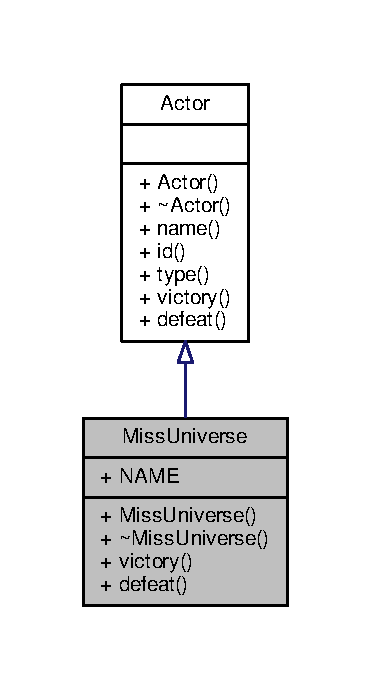
\includegraphics[width=178pt]{classMissUniverse__inherit__graph}
\end{center}
\end{figure}


Collaboration diagram for Miss\+Universe\+:
\nopagebreak
\begin{figure}[H]
\begin{center}
\leavevmode
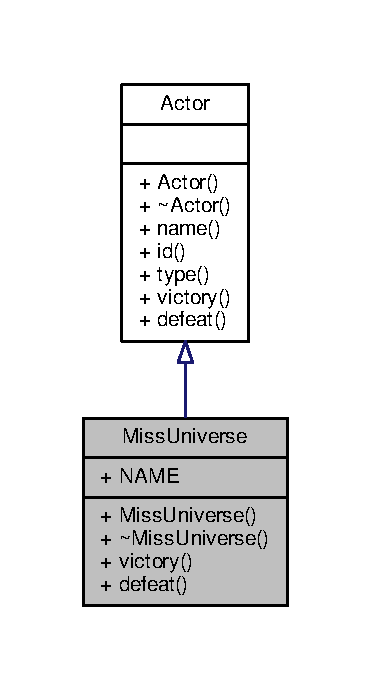
\includegraphics[width=178pt]{classMissUniverse__coll__graph}
\end{center}
\end{figure}
\subsection*{Public Member Functions}
\begin{DoxyCompactItemize}
\item 
\hyperlink{classMissUniverse_ad335e8f67b5c4610f7e5a5f6aaf9b08a}{Miss\+Universe} (unsigned int \hyperlink{classActor_a084438abd4bcb9d5e17b8ad75b0f5984}{id})
\item 
\hyperlink{classMissUniverse_a1a6988dbc5ae8efbef9ec1c9ce4d6cce}{$\sim$\+Miss\+Universe} ()
\item 
virtual std\+::string \hyperlink{classMissUniverse_aac659076d954d5342ba494a993eab2fd}{victory} (const \hyperlink{classActor}{Actor} \&other) const 
\item 
virtual std\+::string \hyperlink{classMissUniverse_af8842e3ec345796fcdadca07a79442b0}{defeat} (const \hyperlink{classActor}{Actor} \&other) const 
\end{DoxyCompactItemize}
\subsection*{Static Public Attributes}
\begin{DoxyCompactItemize}
\item 
static const std\+::string \hyperlink{classMissUniverse_a8030bea29113f33925240bdcce5efd45}{N\+A\+ME} = \char`\"{}Miss\+Universe\char`\"{}
\end{DoxyCompactItemize}
\subsection*{Additional Inherited Members}


\subsection{Detailed Description}
Miss Universe is one of enemies of hero\textquotesingle{}s but basically miss universe are actors. 

\subsection{Constructor \& Destructor Documentation}
\index{Miss\+Universe@{Miss\+Universe}!Miss\+Universe@{Miss\+Universe}}
\index{Miss\+Universe@{Miss\+Universe}!Miss\+Universe@{Miss\+Universe}}
\subsubsection[{\texorpdfstring{Miss\+Universe(unsigned int id)}{MissUniverse(unsigned int id)}}]{\setlength{\rightskip}{0pt plus 5cm}Miss\+Universe\+::\+Miss\+Universe (
\begin{DoxyParamCaption}
\item[{unsigned int}]{id}
\end{DoxyParamCaption}
)}\hypertarget{classMissUniverse_ad335e8f67b5c4610f7e5a5f6aaf9b08a}{}\label{classMissUniverse_ad335e8f67b5c4610f7e5a5f6aaf9b08a}
Create new miss universe 
\begin{DoxyParams}{Parameters}
{\em id} & \+: miss universe actor id \\
\hline
\end{DoxyParams}
\index{Miss\+Universe@{Miss\+Universe}!````~Miss\+Universe@{$\sim$\+Miss\+Universe}}
\index{````~Miss\+Universe@{$\sim$\+Miss\+Universe}!Miss\+Universe@{Miss\+Universe}}
\subsubsection[{\texorpdfstring{$\sim$\+Miss\+Universe()}{~MissUniverse()}}]{\setlength{\rightskip}{0pt plus 5cm}Miss\+Universe\+::$\sim$\+Miss\+Universe (
\begin{DoxyParamCaption}
{}
\end{DoxyParamCaption}
)}\hypertarget{classMissUniverse_a1a6988dbc5ae8efbef9ec1c9ce4d6cce}{}\label{classMissUniverse_a1a6988dbc5ae8efbef9ec1c9ce4d6cce}
Destructor for miss universe 

\subsection{Member Function Documentation}
\index{Miss\+Universe@{Miss\+Universe}!defeat@{defeat}}
\index{defeat@{defeat}!Miss\+Universe@{Miss\+Universe}}
\subsubsection[{\texorpdfstring{defeat(const Actor \&other) const }{defeat(const Actor &other) const }}]{\setlength{\rightskip}{0pt plus 5cm}std\+::string Miss\+Universe\+::defeat (
\begin{DoxyParamCaption}
\item[{const {\bf Actor} \&}]{other}
\end{DoxyParamCaption}
) const\hspace{0.3cm}{\ttfamily [virtual]}}\hypertarget{classMissUniverse_af8842e3ec345796fcdadca07a79442b0}{}\label{classMissUniverse_af8842e3ec345796fcdadca07a79442b0}
message for miss universe defeat over actor actor 
\begin{DoxyParams}{Parameters}
{\em other} & \+: opponent actor \\
\hline
\end{DoxyParams}
\begin{DoxyReturn}{Returns}
defeat message 
\end{DoxyReturn}


Implements \hyperlink{classActor_a0405c30d4ad11809647d2bf4e78026a7}{Actor}.

\index{Miss\+Universe@{Miss\+Universe}!victory@{victory}}
\index{victory@{victory}!Miss\+Universe@{Miss\+Universe}}
\subsubsection[{\texorpdfstring{victory(const Actor \&other) const }{victory(const Actor &other) const }}]{\setlength{\rightskip}{0pt plus 5cm}std\+::string Miss\+Universe\+::victory (
\begin{DoxyParamCaption}
\item[{const {\bf Actor} \&}]{other}
\end{DoxyParamCaption}
) const\hspace{0.3cm}{\ttfamily [virtual]}}\hypertarget{classMissUniverse_aac659076d954d5342ba494a993eab2fd}{}\label{classMissUniverse_aac659076d954d5342ba494a993eab2fd}
message for miss universe winning over other actor 
\begin{DoxyParams}{Parameters}
{\em other} & \+: opponent actor \\
\hline
\end{DoxyParams}
\begin{DoxyReturn}{Returns}
victory message 
\end{DoxyReturn}


Implements \hyperlink{classActor_a1595ffb3d753120a9e74eac0bd69adf1}{Actor}.



\subsection{Member Data Documentation}
\index{Miss\+Universe@{Miss\+Universe}!N\+A\+ME@{N\+A\+ME}}
\index{N\+A\+ME@{N\+A\+ME}!Miss\+Universe@{Miss\+Universe}}
\subsubsection[{\texorpdfstring{N\+A\+ME}{NAME}}]{\setlength{\rightskip}{0pt plus 5cm}const std\+::string Miss\+Universe\+::\+N\+A\+ME = \char`\"{}Miss\+Universe\char`\"{}\hspace{0.3cm}{\ttfamily [static]}}\hypertarget{classMissUniverse_a8030bea29113f33925240bdcce5efd45}{}\label{classMissUniverse_a8030bea29113f33925240bdcce5efd45}


The documentation for this class was generated from the following files\+:\begin{DoxyCompactItemize}
\item 
src/\hyperlink{miss__universe_8h}{miss\+\_\+universe.\+h}\item 
src/\hyperlink{miss__universe_8cpp}{miss\+\_\+universe.\+cpp}\end{DoxyCompactItemize}

\hypertarget{classPolitician}{}\section{Politician Class Reference}
\label{classPolitician}\index{Politician@{Politician}}


{\ttfamily \#include $<$politician.\+h$>$}



Inheritance diagram for Politician\+:
\nopagebreak
\begin{figure}[H]
\begin{center}
\leavevmode
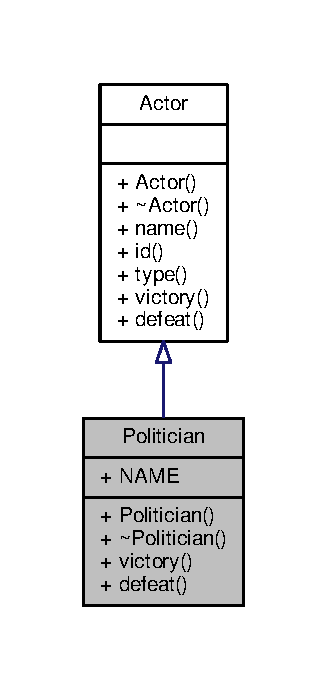
\includegraphics[width=157pt]{classPolitician__inherit__graph}
\end{center}
\end{figure}


Collaboration diagram for Politician\+:
\nopagebreak
\begin{figure}[H]
\begin{center}
\leavevmode
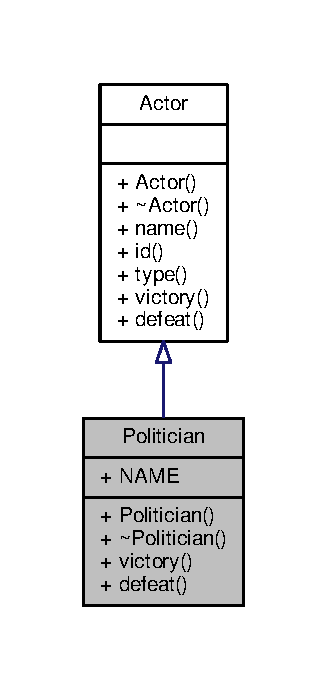
\includegraphics[width=157pt]{classPolitician__coll__graph}
\end{center}
\end{figure}
\subsection*{Public Member Functions}
\begin{DoxyCompactItemize}
\item 
\hyperlink{classPolitician_a334968deab19d05310a8d564299a030a}{Politician} (unsigned int \hyperlink{classActor_a084438abd4bcb9d5e17b8ad75b0f5984}{id})
\item 
\hyperlink{classPolitician_a2ac23dba64f365215b45db3227ef1f6d}{$\sim$\+Politician} ()
\item 
virtual std\+::string \hyperlink{classPolitician_a7428489cb0380195cc5d74faeece6355}{victory} (const \hyperlink{classActor}{Actor} \&other) const 
\item 
virtual std\+::string \hyperlink{classPolitician_a0734a1c1deed35b36b02f83b2c9ee46c}{defeat} (const \hyperlink{classActor}{Actor} \&other) const 
\end{DoxyCompactItemize}
\subsection*{Static Public Attributes}
\begin{DoxyCompactItemize}
\item 
static const std\+::string \hyperlink{classPolitician_a9092b26f16fe1c7b5f88a007ff62db82}{N\+A\+ME} = \char`\"{}Politician\char`\"{}
\end{DoxyCompactItemize}
\subsection*{Additional Inherited Members}


\subsection{Constructor \& Destructor Documentation}
\index{Politician@{Politician}!Politician@{Politician}}
\index{Politician@{Politician}!Politician@{Politician}}
\subsubsection[{\texorpdfstring{Politician(unsigned int id)}{Politician(unsigned int id)}}]{\setlength{\rightskip}{0pt plus 5cm}Politician\+::\+Politician (
\begin{DoxyParamCaption}
\item[{unsigned int}]{id}
\end{DoxyParamCaption}
)}\hypertarget{classPolitician_a334968deab19d05310a8d564299a030a}{}\label{classPolitician_a334968deab19d05310a8d564299a030a}
\index{Politician@{Politician}!````~Politician@{$\sim$\+Politician}}
\index{````~Politician@{$\sim$\+Politician}!Politician@{Politician}}
\subsubsection[{\texorpdfstring{$\sim$\+Politician()}{~Politician()}}]{\setlength{\rightskip}{0pt plus 5cm}Politician\+::$\sim$\+Politician (
\begin{DoxyParamCaption}
{}
\end{DoxyParamCaption}
)}\hypertarget{classPolitician_a2ac23dba64f365215b45db3227ef1f6d}{}\label{classPolitician_a2ac23dba64f365215b45db3227ef1f6d}


\subsection{Member Function Documentation}
\index{Politician@{Politician}!defeat@{defeat}}
\index{defeat@{defeat}!Politician@{Politician}}
\subsubsection[{\texorpdfstring{defeat(const Actor \&other) const }{defeat(const Actor &other) const }}]{\setlength{\rightskip}{0pt plus 5cm}std\+::string Politician\+::defeat (
\begin{DoxyParamCaption}
\item[{const {\bf Actor} \&}]{other}
\end{DoxyParamCaption}
) const\hspace{0.3cm}{\ttfamily [virtual]}}\hypertarget{classPolitician_a0734a1c1deed35b36b02f83b2c9ee46c}{}\label{classPolitician_a0734a1c1deed35b36b02f83b2c9ee46c}


Implements \hyperlink{classActor_a0405c30d4ad11809647d2bf4e78026a7}{Actor}.

\index{Politician@{Politician}!victory@{victory}}
\index{victory@{victory}!Politician@{Politician}}
\subsubsection[{\texorpdfstring{victory(const Actor \&other) const }{victory(const Actor &other) const }}]{\setlength{\rightskip}{0pt plus 5cm}std\+::string Politician\+::victory (
\begin{DoxyParamCaption}
\item[{const {\bf Actor} \&}]{other}
\end{DoxyParamCaption}
) const\hspace{0.3cm}{\ttfamily [virtual]}}\hypertarget{classPolitician_a7428489cb0380195cc5d74faeece6355}{}\label{classPolitician_a7428489cb0380195cc5d74faeece6355}

\begin{DoxyParams}{Parameters}
{\em other} & \\
\hline
\end{DoxyParams}
\begin{DoxyReturn}{Returns}

\end{DoxyReturn}


Implements \hyperlink{classActor_a1595ffb3d753120a9e74eac0bd69adf1}{Actor}.



\subsection{Member Data Documentation}
\index{Politician@{Politician}!N\+A\+ME@{N\+A\+ME}}
\index{N\+A\+ME@{N\+A\+ME}!Politician@{Politician}}
\subsubsection[{\texorpdfstring{N\+A\+ME}{NAME}}]{\setlength{\rightskip}{0pt plus 5cm}const std\+::string Politician\+::\+N\+A\+ME = \char`\"{}Politician\char`\"{}\hspace{0.3cm}{\ttfamily [static]}}\hypertarget{classPolitician_a9092b26f16fe1c7b5f88a007ff62db82}{}\label{classPolitician_a9092b26f16fe1c7b5f88a007ff62db82}


The documentation for this class was generated from the following files\+:\begin{DoxyCompactItemize}
\item 
src/\hyperlink{politician_8h}{politician.\+h}\item 
src/\hyperlink{politician_8cpp}{politician.\+cpp}\end{DoxyCompactItemize}

\hypertarget{classReporter}{}\section{Reporter Class Reference}
\label{classReporter}\index{Reporter@{Reporter}}


{\ttfamily \#include $<$reporter.\+h$>$}



Inheritance diagram for Reporter\+:
\nopagebreak
\begin{figure}[H]
\begin{center}
\leavevmode
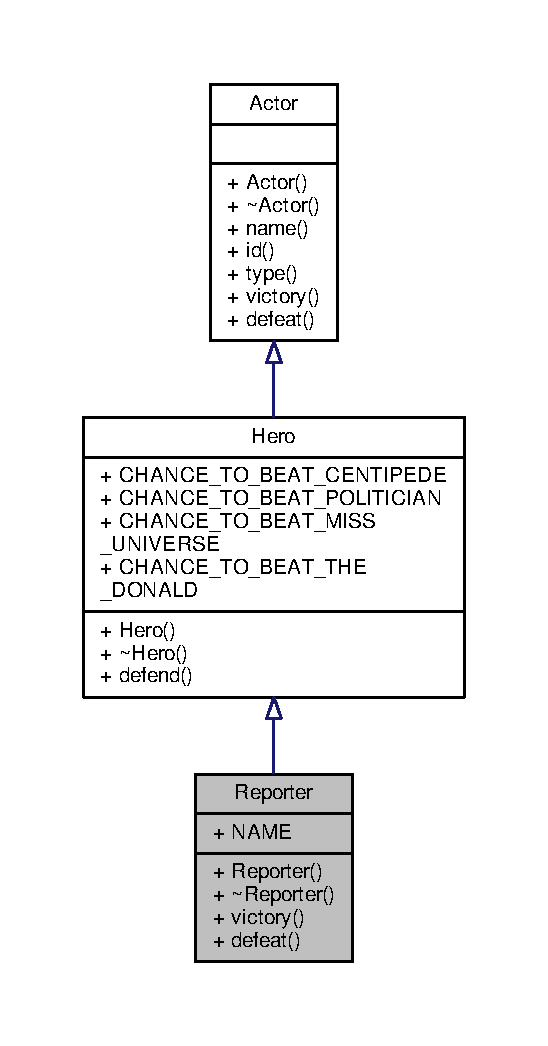
\includegraphics[width=263pt]{classReporter__inherit__graph}
\end{center}
\end{figure}


Collaboration diagram for Reporter\+:
\nopagebreak
\begin{figure}[H]
\begin{center}
\leavevmode
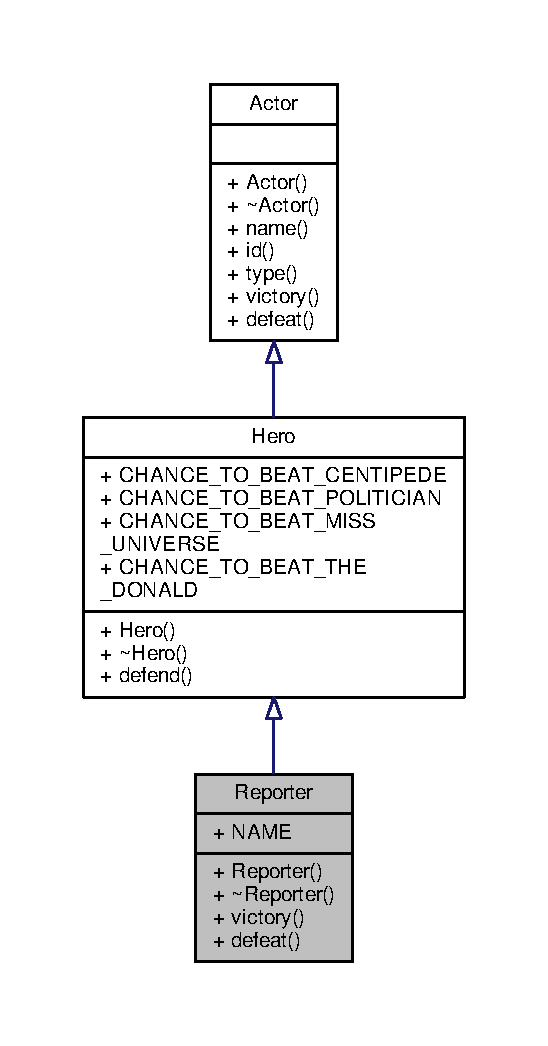
\includegraphics[width=263pt]{classReporter__coll__graph}
\end{center}
\end{figure}
\subsection*{Public Member Functions}
\begin{DoxyCompactItemize}
\item 
\hyperlink{classReporter_a7cfd771737b90ff52c361c1c898a8b6f}{Reporter} (unsigned int \hyperlink{classActor_a084438abd4bcb9d5e17b8ad75b0f5984}{id})
\item 
\hyperlink{classReporter_acbacf4155d5fe9e4a8e833d785e76880}{$\sim$\+Reporter} ()
\item 
virtual std\+::string \hyperlink{classReporter_ac0c496d5f8f3f56c71d2afe6ab53490e}{victory} (const \hyperlink{classActor}{Actor} \&other) const 
\item 
virtual std\+::string \hyperlink{classReporter_a6147cf4ee48d5c81e72538d39c79d228}{defeat} (const \hyperlink{classActor}{Actor} \&other) const 
\end{DoxyCompactItemize}
\subsection*{Static Public Attributes}
\begin{DoxyCompactItemize}
\item 
static const std\+::string \hyperlink{classReporter_a0e02a11312453ea2ad20cbcf32df478d}{N\+A\+ME} = \char`\"{}Reporter\char`\"{}
\end{DoxyCompactItemize}
\subsection*{Additional Inherited Members}


\subsection{Detailed Description}
All Reporters are basically \hyperlink{classHero}{Hero}\textquotesingle{}s 

\subsection{Constructor \& Destructor Documentation}
\index{Reporter@{Reporter}!Reporter@{Reporter}}
\index{Reporter@{Reporter}!Reporter@{Reporter}}
\subsubsection[{\texorpdfstring{Reporter(unsigned int id)}{Reporter(unsigned int id)}}]{\setlength{\rightskip}{0pt plus 5cm}Reporter\+::\+Reporter (
\begin{DoxyParamCaption}
\item[{unsigned int}]{id}
\end{DoxyParamCaption}
)}\hypertarget{classReporter_a7cfd771737b90ff52c361c1c898a8b6f}{}\label{classReporter_a7cfd771737b90ff52c361c1c898a8b6f}
create new reporter 
\begin{DoxyParams}{Parameters}
{\em id} & \+: reporter actor id \\
\hline
\end{DoxyParams}
\index{Reporter@{Reporter}!````~Reporter@{$\sim$\+Reporter}}
\index{````~Reporter@{$\sim$\+Reporter}!Reporter@{Reporter}}
\subsubsection[{\texorpdfstring{$\sim$\+Reporter()}{~Reporter()}}]{\setlength{\rightskip}{0pt plus 5cm}Reporter\+::$\sim$\+Reporter (
\begin{DoxyParamCaption}
{}
\end{DoxyParamCaption}
)}\hypertarget{classReporter_acbacf4155d5fe9e4a8e833d785e76880}{}\label{classReporter_acbacf4155d5fe9e4a8e833d785e76880}
Destructor for \hyperlink{classReporter}{Reporter} 

\subsection{Member Function Documentation}
\index{Reporter@{Reporter}!defeat@{defeat}}
\index{defeat@{defeat}!Reporter@{Reporter}}
\subsubsection[{\texorpdfstring{defeat(const Actor \&other) const }{defeat(const Actor &other) const }}]{\setlength{\rightskip}{0pt plus 5cm}std\+::string Reporter\+::defeat (
\begin{DoxyParamCaption}
\item[{const {\bf Actor} \&}]{other}
\end{DoxyParamCaption}
) const\hspace{0.3cm}{\ttfamily [virtual]}}\hypertarget{classReporter_a6147cf4ee48d5c81e72538d39c79d228}{}\label{classReporter_a6147cf4ee48d5c81e72538d39c79d228}
message for reporter defeat over other actor 
\begin{DoxyParams}{Parameters}
{\em other} & \+: opponent actor \\
\hline
\end{DoxyParams}
\begin{DoxyReturn}{Returns}
\+: message for defeat 
\end{DoxyReturn}


Implements \hyperlink{classActor_a0405c30d4ad11809647d2bf4e78026a7}{Actor}.

\index{Reporter@{Reporter}!victory@{victory}}
\index{victory@{victory}!Reporter@{Reporter}}
\subsubsection[{\texorpdfstring{victory(const Actor \&other) const }{victory(const Actor &other) const }}]{\setlength{\rightskip}{0pt plus 5cm}std\+::string Reporter\+::victory (
\begin{DoxyParamCaption}
\item[{const {\bf Actor} \&}]{other}
\end{DoxyParamCaption}
) const\hspace{0.3cm}{\ttfamily [virtual]}}\hypertarget{classReporter_ac0c496d5f8f3f56c71d2afe6ab53490e}{}\label{classReporter_ac0c496d5f8f3f56c71d2afe6ab53490e}
message for reporter victory over other actor 
\begin{DoxyParams}{Parameters}
{\em other} & \+: opponent actor \\
\hline
\end{DoxyParams}
\begin{DoxyReturn}{Returns}
\+: message for victory 
\end{DoxyReturn}


Implements \hyperlink{classActor_a1595ffb3d753120a9e74eac0bd69adf1}{Actor}.



\subsection{Member Data Documentation}
\index{Reporter@{Reporter}!N\+A\+ME@{N\+A\+ME}}
\index{N\+A\+ME@{N\+A\+ME}!Reporter@{Reporter}}
\subsubsection[{\texorpdfstring{N\+A\+ME}{NAME}}]{\setlength{\rightskip}{0pt plus 5cm}const std\+::string Reporter\+::\+N\+A\+ME = \char`\"{}Reporter\char`\"{}\hspace{0.3cm}{\ttfamily [static]}}\hypertarget{classReporter_a0e02a11312453ea2ad20cbcf32df478d}{}\label{classReporter_a0e02a11312453ea2ad20cbcf32df478d}


The documentation for this class was generated from the following files\+:\begin{DoxyCompactItemize}
\item 
src/\hyperlink{reporter_8h}{reporter.\+h}\item 
src/\hyperlink{reporter_8cpp}{reporter.\+cpp}\end{DoxyCompactItemize}

\hypertarget{classRNG}{}\section{R\+NG Class Reference}
\label{classRNG}\index{R\+NG@{R\+NG}}


{\ttfamily \#include $<$rng.\+h$>$}



Collaboration diagram for R\+NG\+:
\nopagebreak
\begin{figure}[H]
\begin{center}
\leavevmode
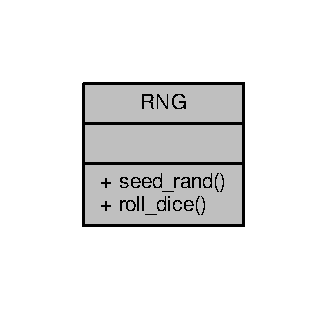
\includegraphics[width=157pt]{classRNG__coll__graph}
\end{center}
\end{figure}
\subsection*{Static Public Member Functions}
\begin{DoxyCompactItemize}
\item 
static void \hyperlink{classRNG_ab860f171afa8f937eccba29a8575f55a}{seed\+\_\+rand} (int seed)
\item 
static bool \hyperlink{classRNG_ad3340707ef6f70eeb2923572c2839b02}{roll\+\_\+dice} (const std\+::string \&a, const std\+::string \&b, int winning\+\_\+chances)
\end{DoxyCompactItemize}


\subsection{Detailed Description}
A pseudo random number generator that uses a simple linear congruential generator\+:

\href{https://rosettacode.org/wiki/Linear_congruential_generator}{\tt https\+://rosettacode.\+org/wiki/\+Linear\+\_\+congruential\+\_\+generator}

\begin{DoxyAuthor}{Author}
Sean Strout @ R\+IT CS 
\end{DoxyAuthor}


\subsection{Member Function Documentation}
\index{R\+NG@{R\+NG}!roll\+\_\+dice@{roll\+\_\+dice}}
\index{roll\+\_\+dice@{roll\+\_\+dice}!R\+NG@{R\+NG}}
\subsubsection[{\texorpdfstring{roll\+\_\+dice(const std\+::string \&a, const std\+::string \&b, int winning\+\_\+chances)}{roll_dice(const std::string &a, const std::string &b, int winning_chances)}}]{\setlength{\rightskip}{0pt plus 5cm}bool R\+N\+G\+::roll\+\_\+dice (
\begin{DoxyParamCaption}
\item[{const std\+::string \&}]{a, }
\item[{const std\+::string \&}]{b, }
\item[{int}]{winning\+\_\+chances}
\end{DoxyParamCaption}
)\hspace{0.3cm}{\ttfamily [static]}}\hypertarget{classRNG_ad3340707ef6f70eeb2923572c2839b02}{}\label{classRNG_ad3340707ef6f70eeb2923572c2839b02}
a rolls the dice against b, with a\textquotesingle{}s chance to defeat b as 0..winning\+\_\+chances-\/1. It prints out the message where \{result\} is between 0..99 inclusively.

\{a\} rolls a \{result\} against \{b\}


\begin{DoxyParams}{Parameters}
{\em a} & the dice roller \\
\hline
{\em b} & who the dice roller is rolling against \\
\hline
{\em winning\+\_\+chances} & a value between 0 and 100, inclusively, as a\textquotesingle{}s chance to beat b \\
\hline
\end{DoxyParams}
\begin{DoxyReturn}{Returns}
whether a beat b or not 
\end{DoxyReturn}
\index{R\+NG@{R\+NG}!seed\+\_\+rand@{seed\+\_\+rand}}
\index{seed\+\_\+rand@{seed\+\_\+rand}!R\+NG@{R\+NG}}
\subsubsection[{\texorpdfstring{seed\+\_\+rand(int seed)}{seed_rand(int seed)}}]{\setlength{\rightskip}{0pt plus 5cm}void R\+N\+G\+::seed\+\_\+rand (
\begin{DoxyParamCaption}
\item[{int}]{seed}
\end{DoxyParamCaption}
)\hspace{0.3cm}{\ttfamily [static]}}\hypertarget{classRNG_ab860f171afa8f937eccba29a8575f55a}{}\label{classRNG_ab860f171afa8f937eccba29a8575f55a}
Seed the random number generator so roll\+\_\+dice has predictable output.


\begin{DoxyParams}{Parameters}
{\em seed} & seed value \\
\hline
\end{DoxyParams}


The documentation for this class was generated from the following files\+:\begin{DoxyCompactItemize}
\item 
src/\hyperlink{rng_8h}{rng.\+h}\item 
src/\hyperlink{rng_8cpp}{rng.\+cpp}\end{DoxyCompactItemize}

\hypertarget{classSJW}{}\section{S\+JW Class Reference}
\label{classSJW}\index{S\+JW@{S\+JW}}


{\ttfamily \#include $<$sjw.\+h$>$}



Inheritance diagram for S\+JW\+:
\nopagebreak
\begin{figure}[H]
\begin{center}
\leavevmode
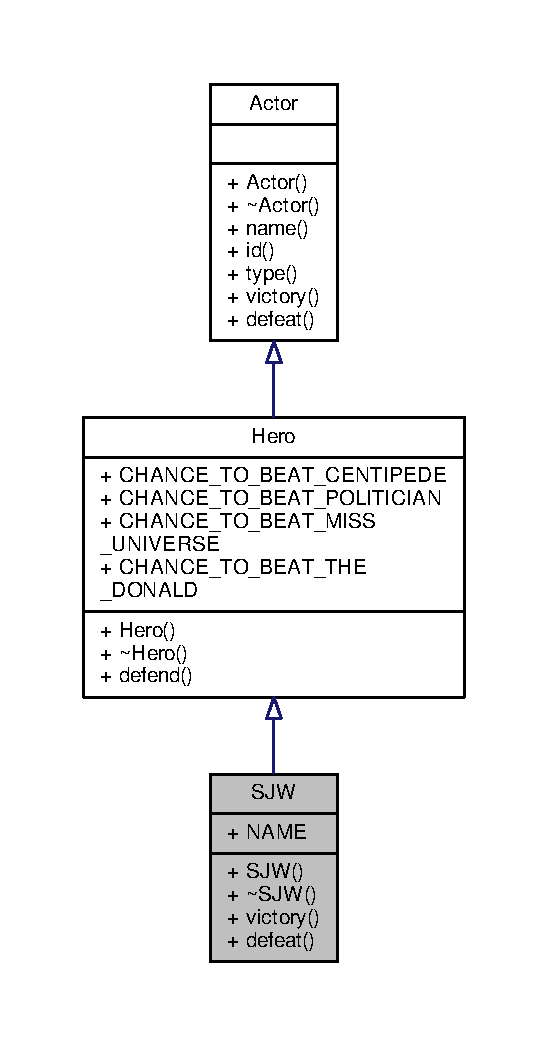
\includegraphics[width=263pt]{classSJW__inherit__graph}
\end{center}
\end{figure}


Collaboration diagram for S\+JW\+:
\nopagebreak
\begin{figure}[H]
\begin{center}
\leavevmode
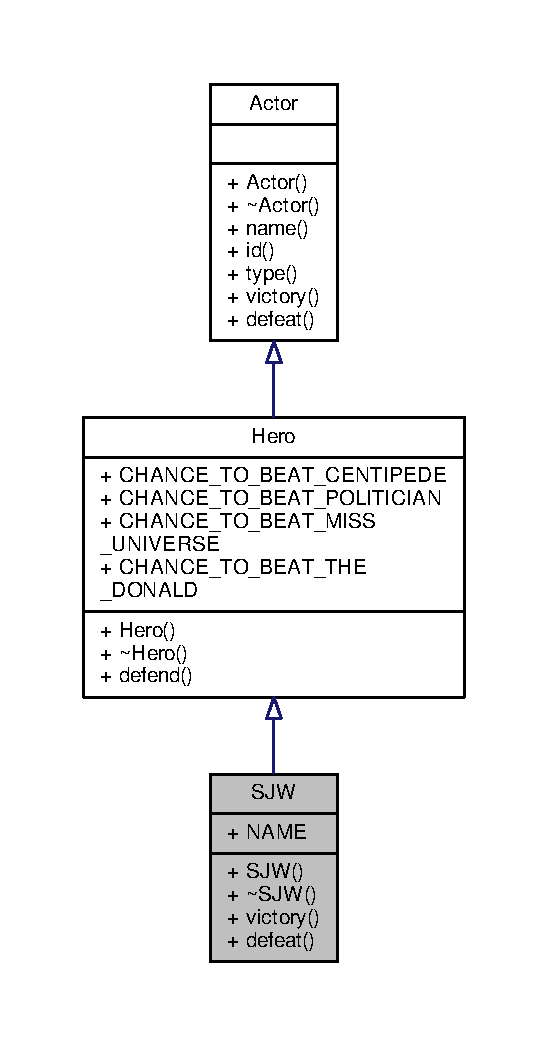
\includegraphics[width=263pt]{classSJW__coll__graph}
\end{center}
\end{figure}
\subsection*{Public Member Functions}
\begin{DoxyCompactItemize}
\item 
\hyperlink{classSJW_aee0f414b8da298a625c303173cd9bfe2}{S\+JW} (unsigned int \hyperlink{classActor_a084438abd4bcb9d5e17b8ad75b0f5984}{id})
\item 
\hyperlink{classSJW_a28fa43a9925b7308b3f06b004510abeb}{$\sim$\+S\+JW} ()
\item 
virtual std\+::string \hyperlink{classSJW_af9bffa85da9c04559f38210f11a80c1d}{victory} (const \hyperlink{classActor}{Actor} \&other) const 
\item 
virtual std\+::string \hyperlink{classSJW_a04d480d0bedb684591a1a14d41b93257}{defeat} (const \hyperlink{classActor}{Actor} \&other) const 
\end{DoxyCompactItemize}
\subsection*{Static Public Attributes}
\begin{DoxyCompactItemize}
\item 
static const std\+::string \hyperlink{classSJW_a38d0a4a884536b96c3c9e7b5c32bf0fb}{N\+A\+ME} = \char`\"{}S\+JW\char`\"{}
\end{DoxyCompactItemize}
\subsection*{Additional Inherited Members}


\subsection{Detailed Description}
All \hyperlink{classSJW}{S\+JW}\textquotesingle{}s are basically \hyperlink{classHero}{Hero}\textquotesingle{}s 

\subsection{Constructor \& Destructor Documentation}
\index{S\+JW@{S\+JW}!S\+JW@{S\+JW}}
\index{S\+JW@{S\+JW}!S\+JW@{S\+JW}}
\subsubsection[{\texorpdfstring{S\+J\+W(unsigned int id)}{SJW(unsigned int id)}}]{\setlength{\rightskip}{0pt plus 5cm}S\+J\+W\+::\+S\+JW (
\begin{DoxyParamCaption}
\item[{unsigned int}]{id}
\end{DoxyParamCaption}
)}\hypertarget{classSJW_aee0f414b8da298a625c303173cd9bfe2}{}\label{classSJW_aee0f414b8da298a625c303173cd9bfe2}
create new \hyperlink{classSJW}{S\+JW} \hyperlink{classHero}{Hero} 
\begin{DoxyParams}{Parameters}
{\em id} & \+: \hyperlink{classSJW}{S\+JW} id \\
\hline
\end{DoxyParams}
\index{S\+JW@{S\+JW}!````~S\+JW@{$\sim$\+S\+JW}}
\index{````~S\+JW@{$\sim$\+S\+JW}!S\+JW@{S\+JW}}
\subsubsection[{\texorpdfstring{$\sim$\+S\+J\+W()}{~SJW()}}]{\setlength{\rightskip}{0pt plus 5cm}S\+J\+W\+::$\sim$\+S\+JW (
\begin{DoxyParamCaption}
{}
\end{DoxyParamCaption}
)}\hypertarget{classSJW_a28fa43a9925b7308b3f06b004510abeb}{}\label{classSJW_a28fa43a9925b7308b3f06b004510abeb}
Destructor for \hyperlink{classSJW}{S\+JW} 

\subsection{Member Function Documentation}
\index{S\+JW@{S\+JW}!defeat@{defeat}}
\index{defeat@{defeat}!S\+JW@{S\+JW}}
\subsubsection[{\texorpdfstring{defeat(const Actor \&other) const }{defeat(const Actor &other) const }}]{\setlength{\rightskip}{0pt plus 5cm}std\+::string S\+J\+W\+::defeat (
\begin{DoxyParamCaption}
\item[{const {\bf Actor} \&}]{other}
\end{DoxyParamCaption}
) const\hspace{0.3cm}{\ttfamily [virtual]}}\hypertarget{classSJW_a04d480d0bedb684591a1a14d41b93257}{}\label{classSJW_a04d480d0bedb684591a1a14d41b93257}
message for \hyperlink{classSJW}{S\+JW} hero defeat over other actor 
\begin{DoxyParams}{Parameters}
{\em other} & \+: opponent actor \\
\hline
\end{DoxyParams}
\begin{DoxyReturn}{Returns}
\+: message for defeat 
\end{DoxyReturn}


Implements \hyperlink{classActor_a0405c30d4ad11809647d2bf4e78026a7}{Actor}.

\index{S\+JW@{S\+JW}!victory@{victory}}
\index{victory@{victory}!S\+JW@{S\+JW}}
\subsubsection[{\texorpdfstring{victory(const Actor \&other) const }{victory(const Actor &other) const }}]{\setlength{\rightskip}{0pt plus 5cm}std\+::string S\+J\+W\+::victory (
\begin{DoxyParamCaption}
\item[{const {\bf Actor} \&}]{other}
\end{DoxyParamCaption}
) const\hspace{0.3cm}{\ttfamily [virtual]}}\hypertarget{classSJW_af9bffa85da9c04559f38210f11a80c1d}{}\label{classSJW_af9bffa85da9c04559f38210f11a80c1d}
message for \hyperlink{classSJW}{S\+JW} hero victory over other actor 
\begin{DoxyParams}{Parameters}
{\em other} & \+: opponent actor \\
\hline
\end{DoxyParams}
\begin{DoxyReturn}{Returns}
\+: message for victory 
\end{DoxyReturn}


Implements \hyperlink{classActor_a1595ffb3d753120a9e74eac0bd69adf1}{Actor}.



\subsection{Member Data Documentation}
\index{S\+JW@{S\+JW}!N\+A\+ME@{N\+A\+ME}}
\index{N\+A\+ME@{N\+A\+ME}!S\+JW@{S\+JW}}
\subsubsection[{\texorpdfstring{N\+A\+ME}{NAME}}]{\setlength{\rightskip}{0pt plus 5cm}const std\+::string S\+J\+W\+::\+N\+A\+ME = \char`\"{}S\+JW\char`\"{}\hspace{0.3cm}{\ttfamily [static]}}\hypertarget{classSJW_a38d0a4a884536b96c3c9e7b5c32bf0fb}{}\label{classSJW_a38d0a4a884536b96c3c9e7b5c32bf0fb}


The documentation for this class was generated from the following files\+:\begin{DoxyCompactItemize}
\item 
src/\hyperlink{sjw_8h}{sjw.\+h}\item 
src/\hyperlink{sjw_8cpp}{sjw.\+cpp}\end{DoxyCompactItemize}

\hypertarget{classTheDonald}{}\section{The\+Donald Class Reference}
\label{classTheDonald}\index{The\+Donald@{The\+Donald}}


{\ttfamily \#include $<$the\+\_\+donald.\+h$>$}



Inheritance diagram for The\+Donald\+:
\nopagebreak
\begin{figure}[H]
\begin{center}
\leavevmode
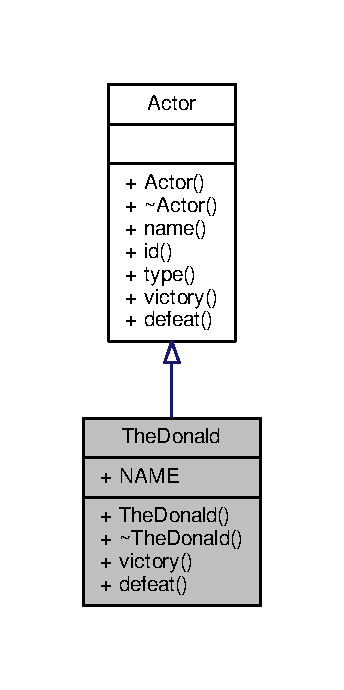
\includegraphics[width=165pt]{classTheDonald__inherit__graph}
\end{center}
\end{figure}


Collaboration diagram for The\+Donald\+:
\nopagebreak
\begin{figure}[H]
\begin{center}
\leavevmode
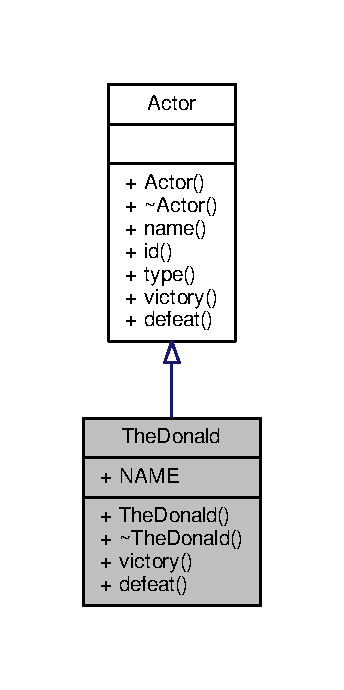
\includegraphics[width=165pt]{classTheDonald__coll__graph}
\end{center}
\end{figure}
\subsection*{Public Member Functions}
\begin{DoxyCompactItemize}
\item 
\hyperlink{classTheDonald_a3e3d985e27af763356a7936d8bf190d8}{The\+Donald} (unsigned int \hyperlink{classActor_a084438abd4bcb9d5e17b8ad75b0f5984}{id})
\item 
\hyperlink{classTheDonald_a0c0193bf480aceaaebc3598da56409e8}{$\sim$\+The\+Donald} ()
\item 
virtual std\+::string \hyperlink{classTheDonald_abee1d5bb4910c657ffd41fc745298cdc}{victory} (const \hyperlink{classActor}{Actor} \&other) const 
\item 
virtual std\+::string \hyperlink{classTheDonald_ac6920f6026c3b0d91afbce90f6f07fad}{defeat} (const \hyperlink{classActor}{Actor} \&other) const 
\end{DoxyCompactItemize}
\subsection*{Static Public Attributes}
\begin{DoxyCompactItemize}
\item 
static const std\+::string \hyperlink{classTheDonald_a5524e0abfd4ea1eb4f22f526f4583732}{N\+A\+ME} = \char`\"{}The Donald\char`\"{}
\end{DoxyCompactItemize}
\subsection*{Additional Inherited Members}


\subsection{Detailed Description}
Donal is one of the main actor 

\subsection{Constructor \& Destructor Documentation}
\index{The\+Donald@{The\+Donald}!The\+Donald@{The\+Donald}}
\index{The\+Donald@{The\+Donald}!The\+Donald@{The\+Donald}}
\subsubsection[{\texorpdfstring{The\+Donald(unsigned int id)}{TheDonald(unsigned int id)}}]{\setlength{\rightskip}{0pt plus 5cm}The\+Donald\+::\+The\+Donald (
\begin{DoxyParamCaption}
\item[{unsigned int}]{id = {\ttfamily 1}}
\end{DoxyParamCaption}
)}\hypertarget{classTheDonald_a3e3d985e27af763356a7936d8bf190d8}{}\label{classTheDonald_a3e3d985e27af763356a7936d8bf190d8}
create new donald 
\begin{DoxyParams}{Parameters}
{\em id} & \+: donald\textquotesingle{}s actor id \\
\hline
\end{DoxyParams}
\index{The\+Donald@{The\+Donald}!````~The\+Donald@{$\sim$\+The\+Donald}}
\index{````~The\+Donald@{$\sim$\+The\+Donald}!The\+Donald@{The\+Donald}}
\subsubsection[{\texorpdfstring{$\sim$\+The\+Donald()}{~TheDonald()}}]{\setlength{\rightskip}{0pt plus 5cm}The\+Donald\+::$\sim$\+The\+Donald (
\begin{DoxyParamCaption}
{}
\end{DoxyParamCaption}
)}\hypertarget{classTheDonald_a0c0193bf480aceaaebc3598da56409e8}{}\label{classTheDonald_a0c0193bf480aceaaebc3598da56409e8}
Destrctr for donald 

\subsection{Member Function Documentation}
\index{The\+Donald@{The\+Donald}!defeat@{defeat}}
\index{defeat@{defeat}!The\+Donald@{The\+Donald}}
\subsubsection[{\texorpdfstring{defeat(const Actor \&other) const }{defeat(const Actor &other) const }}]{\setlength{\rightskip}{0pt plus 5cm}std\+::string The\+Donald\+::defeat (
\begin{DoxyParamCaption}
\item[{const {\bf Actor} \&}]{other}
\end{DoxyParamCaption}
) const\hspace{0.3cm}{\ttfamily [virtual]}}\hypertarget{classTheDonald_ac6920f6026c3b0d91afbce90f6f07fad}{}\label{classTheDonald_ac6920f6026c3b0d91afbce90f6f07fad}
message for Donald defeat over other actor 
\begin{DoxyParams}{Parameters}
{\em other} & \+: opponent actor \\
\hline
\end{DoxyParams}
\begin{DoxyReturn}{Returns}
\+: message for defeat 
\end{DoxyReturn}


Implements \hyperlink{classActor_a0405c30d4ad11809647d2bf4e78026a7}{Actor}.

\index{The\+Donald@{The\+Donald}!victory@{victory}}
\index{victory@{victory}!The\+Donald@{The\+Donald}}
\subsubsection[{\texorpdfstring{victory(const Actor \&other) const }{victory(const Actor &other) const }}]{\setlength{\rightskip}{0pt plus 5cm}std\+::string The\+Donald\+::victory (
\begin{DoxyParamCaption}
\item[{const {\bf Actor} \&}]{other}
\end{DoxyParamCaption}
) const\hspace{0.3cm}{\ttfamily [virtual]}}\hypertarget{classTheDonald_abee1d5bb4910c657ffd41fc745298cdc}{}\label{classTheDonald_abee1d5bb4910c657ffd41fc745298cdc}
message for Donald victory over other actor 
\begin{DoxyParams}{Parameters}
{\em other} & \+: opponent actor \\
\hline
\end{DoxyParams}
\begin{DoxyReturn}{Returns}
\+: message for victory 
\end{DoxyReturn}


Implements \hyperlink{classActor_a1595ffb3d753120a9e74eac0bd69adf1}{Actor}.



\subsection{Member Data Documentation}
\index{The\+Donald@{The\+Donald}!N\+A\+ME@{N\+A\+ME}}
\index{N\+A\+ME@{N\+A\+ME}!The\+Donald@{The\+Donald}}
\subsubsection[{\texorpdfstring{N\+A\+ME}{NAME}}]{\setlength{\rightskip}{0pt plus 5cm}const std\+::string The\+Donald\+::\+N\+A\+ME = \char`\"{}The Donald\char`\"{}\hspace{0.3cm}{\ttfamily [static]}}\hypertarget{classTheDonald_a5524e0abfd4ea1eb4f22f526f4583732}{}\label{classTheDonald_a5524e0abfd4ea1eb4f22f526f4583732}


The documentation for this class was generated from the following files\+:\begin{DoxyCompactItemize}
\item 
src/\hyperlink{the__donald_8h}{the\+\_\+donald.\+h}\item 
src/\hyperlink{the__donald_8cpp}{the\+\_\+donald.\+cpp}\end{DoxyCompactItemize}

\hypertarget{classTrumpTower}{}\section{Trump\+Tower Class Reference}
\label{classTrumpTower}\index{Trump\+Tower@{Trump\+Tower}}


{\ttfamily \#include $<$trump\+\_\+tower.\+h$>$}



Collaboration diagram for Trump\+Tower\+:
\nopagebreak
\begin{figure}[H]
\begin{center}
\leavevmode
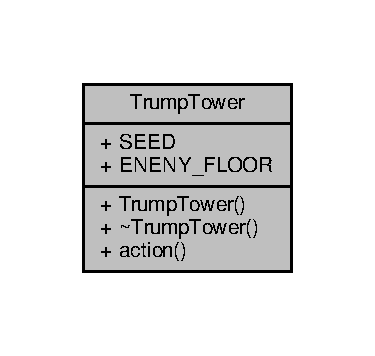
\includegraphics[width=180pt]{classTrumpTower__coll__graph}
\end{center}
\end{figure}
\subsection*{Public Member Functions}
\begin{DoxyCompactItemize}
\item 
\hyperlink{classTrumpTower_a289ef64fd3602f7df558eeeda36ab237}{Trump\+Tower} (unsigned long num\+S\+J\+Ws, unsigned long num\+Reporters, unsigned long num\+Centipedes, unsigned long num\+Politicians, unsigned long num\+Miss\+Universes)
\item 
virtual \hyperlink{classTrumpTower_aa9ac742a7e39584d63207cbff1712c21}{$\sim$\+Trump\+Tower} ()
\item 
void \hyperlink{classTrumpTower_a2eb063d540d428f2f41bf5264e67c283}{action} ()
\end{DoxyCompactItemize}
\subsection*{Static Public Attributes}
\begin{DoxyCompactItemize}
\item 
static const int \hyperlink{classTrumpTower_a7207ac5ab137b0fc2ff175eec3592fec}{S\+E\+ED} = 0
\item 
static const unsigned int \hyperlink{classTrumpTower_aae8db3b60d8960faf570d0e35ba195d6}{E\+N\+E\+N\+Y\+\_\+\+F\+L\+O\+OR} = 13
\end{DoxyCompactItemize}


\subsection{Detailed Description}
Trump Tower is were all the work happens, hero\textquotesingle{}s fight enemies to rescue reporters, reporters fight donald trump. All winning reporters all taken by chopper and other loosing reporters with heros are sent to wahambulance. 

\subsection{Constructor \& Destructor Documentation}
\index{Trump\+Tower@{Trump\+Tower}!Trump\+Tower@{Trump\+Tower}}
\index{Trump\+Tower@{Trump\+Tower}!Trump\+Tower@{Trump\+Tower}}
\subsubsection[{\texorpdfstring{Trump\+Tower(unsigned long num\+S\+J\+Ws, unsigned long num\+Reporters, unsigned long num\+Centipedes, unsigned long num\+Politicians, unsigned long num\+Miss\+Universes)}{TrumpTower(unsigned long numSJWs, unsigned long numReporters, unsigned long numCentipedes, unsigned long numPoliticians, unsigned long numMissUniverses)}}]{\setlength{\rightskip}{0pt plus 5cm}Trump\+Tower\+::\+Trump\+Tower (
\begin{DoxyParamCaption}
\item[{unsigned long}]{num\+S\+J\+Ws, }
\item[{unsigned long}]{num\+Reporters, }
\item[{unsigned long}]{num\+Centipedes, }
\item[{unsigned long}]{num\+Politicians, }
\item[{unsigned long}]{num\+Miss\+Universes}
\end{DoxyParamCaption}
)}\hypertarget{classTrumpTower_a289ef64fd3602f7df558eeeda36ab237}{}\label{classTrumpTower_a289ef64fd3602f7df558eeeda36ab237}
Construct \hyperlink{classTrumpTower}{Trump\+Tower} with heros, reporters, enemies and donald trump 
\begin{DoxyParams}{Parameters}
{\em num\+S\+J\+Ws} & \+: number of \hyperlink{classSJW}{S\+JW} heros to be initiated \\
\hline
{\em num\+Reporters} & \+: number of Reporters to be initiated \\
\hline
{\em num\+Centipedes} & \+: number of enemy centipedes to be initiated \\
\hline
{\em num\+Politicians} & \+: number of enemy politicians to be initiated \\
\hline
{\em num\+Miss\+Universes} & \+: number of enemy miss universes to be initiated \\
\hline
\end{DoxyParams}
\index{Trump\+Tower@{Trump\+Tower}!````~Trump\+Tower@{$\sim$\+Trump\+Tower}}
\index{````~Trump\+Tower@{$\sim$\+Trump\+Tower}!Trump\+Tower@{Trump\+Tower}}
\subsubsection[{\texorpdfstring{$\sim$\+Trump\+Tower()}{~TrumpTower()}}]{\setlength{\rightskip}{0pt plus 5cm}Trump\+Tower\+::$\sim$\+Trump\+Tower (
\begin{DoxyParamCaption}
{}
\end{DoxyParamCaption}
)\hspace{0.3cm}{\ttfamily [virtual]}}\hypertarget{classTrumpTower_aa9ac742a7e39584d63207cbff1712c21}{}\label{classTrumpTower_aa9ac742a7e39584d63207cbff1712c21}
Kill(\+Delete) everyone inside trump tower. delete all heros, reporters, enemies. 

\subsection{Member Function Documentation}
\index{Trump\+Tower@{Trump\+Tower}!action@{action}}
\index{action@{action}!Trump\+Tower@{Trump\+Tower}}
\subsubsection[{\texorpdfstring{action()}{action()}}]{\setlength{\rightskip}{0pt plus 5cm}void Trump\+Tower\+::action (
\begin{DoxyParamCaption}
{}
\end{DoxyParamCaption}
)}\hypertarget{classTrumpTower_a2eb063d540d428f2f41bf5264e67c283}{}\label{classTrumpTower_a2eb063d540d428f2f41bf5264e67c283}
Once all the actors are ready, the movie acton starts 

\subsection{Member Data Documentation}
\index{Trump\+Tower@{Trump\+Tower}!E\+N\+E\+N\+Y\+\_\+\+F\+L\+O\+OR@{E\+N\+E\+N\+Y\+\_\+\+F\+L\+O\+OR}}
\index{E\+N\+E\+N\+Y\+\_\+\+F\+L\+O\+OR@{E\+N\+E\+N\+Y\+\_\+\+F\+L\+O\+OR}!Trump\+Tower@{Trump\+Tower}}
\subsubsection[{\texorpdfstring{E\+N\+E\+N\+Y\+\_\+\+F\+L\+O\+OR}{ENENY_FLOOR}}]{\setlength{\rightskip}{0pt plus 5cm}const unsigned int Trump\+Tower\+::\+E\+N\+E\+N\+Y\+\_\+\+F\+L\+O\+OR = 13\hspace{0.3cm}{\ttfamily [static]}}\hypertarget{classTrumpTower_aae8db3b60d8960faf570d0e35ba195d6}{}\label{classTrumpTower_aae8db3b60d8960faf570d0e35ba195d6}
\index{Trump\+Tower@{Trump\+Tower}!S\+E\+ED@{S\+E\+ED}}
\index{S\+E\+ED@{S\+E\+ED}!Trump\+Tower@{Trump\+Tower}}
\subsubsection[{\texorpdfstring{S\+E\+ED}{SEED}}]{\setlength{\rightskip}{0pt plus 5cm}const int Trump\+Tower\+::\+S\+E\+ED = 0\hspace{0.3cm}{\ttfamily [static]}}\hypertarget{classTrumpTower_a7207ac5ab137b0fc2ff175eec3592fec}{}\label{classTrumpTower_a7207ac5ab137b0fc2ff175eec3592fec}


The documentation for this class was generated from the following files\+:\begin{DoxyCompactItemize}
\item 
src/\hyperlink{trump__tower_8h}{trump\+\_\+tower.\+h}\item 
src/\hyperlink{trump__tower_8cpp}{trump\+\_\+tower.\+cpp}\end{DoxyCompactItemize}

\hypertarget{classTTException}{}\section{T\+T\+Exception Class Reference}
\label{classTTException}\index{T\+T\+Exception@{T\+T\+Exception}}


{\ttfamily \#include $<$tt\+\_\+exception.\+h$>$}



Inheritance diagram for T\+T\+Exception\+:
\nopagebreak
\begin{figure}[H]
\begin{center}
\leavevmode
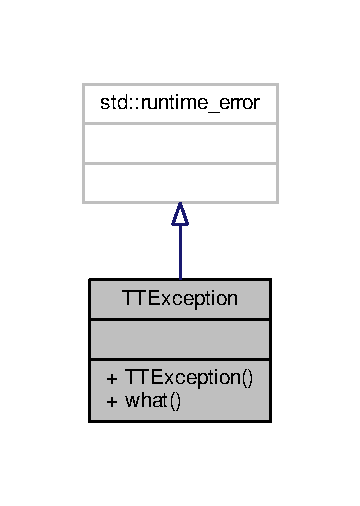
\includegraphics[width=173pt]{classTTException__inherit__graph}
\end{center}
\end{figure}


Collaboration diagram for T\+T\+Exception\+:
\nopagebreak
\begin{figure}[H]
\begin{center}
\leavevmode
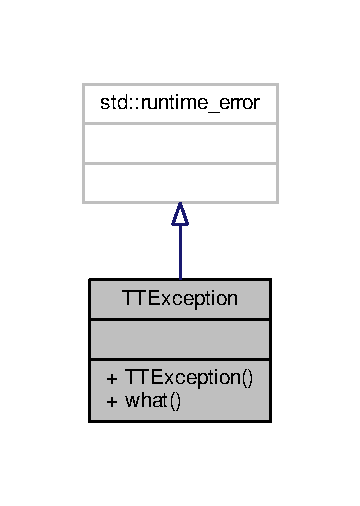
\includegraphics[width=173pt]{classTTException__coll__graph}
\end{center}
\end{figure}
\subsection*{Public Member Functions}
\begin{DoxyCompactItemize}
\item 
\hyperlink{classTTException_a1a7415151aeb69b2a0ce2c150c63e46a}{T\+T\+Exception} (const char $\ast$msg)
\item 
virtual const char $\ast$ \hyperlink{classTTException_a89fb8e8d64f5a98813956334c5179c1f}{what} () const   throw ()
\end{DoxyCompactItemize}


\subsection{Detailed Description}
Exception class from run time error 

\subsection{Constructor \& Destructor Documentation}
\index{T\+T\+Exception@{T\+T\+Exception}!T\+T\+Exception@{T\+T\+Exception}}
\index{T\+T\+Exception@{T\+T\+Exception}!T\+T\+Exception@{T\+T\+Exception}}
\subsubsection[{\texorpdfstring{T\+T\+Exception(const char $\ast$msg)}{TTException(const char *msg)}}]{\setlength{\rightskip}{0pt plus 5cm}T\+T\+Exception\+::\+T\+T\+Exception (
\begin{DoxyParamCaption}
\item[{const char $\ast$}]{msg}
\end{DoxyParamCaption}
)\hspace{0.3cm}{\ttfamily [inline]}}\hypertarget{classTTException_a1a7415151aeb69b2a0ce2c150c63e46a}{}\label{classTTException_a1a7415151aeb69b2a0ce2c150c63e46a}
create a execption class with the message 
\begin{DoxyParams}{Parameters}
{\em msg} & \+: exception message \\
\hline
\end{DoxyParams}


\subsection{Member Function Documentation}
\index{T\+T\+Exception@{T\+T\+Exception}!what@{what}}
\index{what@{what}!T\+T\+Exception@{T\+T\+Exception}}
\subsubsection[{\texorpdfstring{what() const }{what() const }}]{\setlength{\rightskip}{0pt plus 5cm}virtual const char$\ast$ T\+T\+Exception\+::what (
\begin{DoxyParamCaption}
{}
\end{DoxyParamCaption}
) const throw  ) \hspace{0.3cm}{\ttfamily [inline]}, {\ttfamily [virtual]}}\hypertarget{classTTException_a89fb8e8d64f5a98813956334c5179c1f}{}\label{classTTException_a89fb8e8d64f5a98813956334c5179c1f}
Exception message throwable \begin{DoxyReturn}{Returns}
\+: exception message 
\end{DoxyReturn}


The documentation for this class was generated from the following file\+:\begin{DoxyCompactItemize}
\item 
src/\hyperlink{tt__exception_8h}{tt\+\_\+exception.\+h}\end{DoxyCompactItemize}

\chapter{File Documentation}
\hypertarget{actor_8cpp}{}\section{src/actor.cpp File Reference}
\label{actor_8cpp}\index{src/actor.\+cpp@{src/actor.\+cpp}}
{\ttfamily \#include \char`\"{}actor.\+h\char`\"{}}\\*
{\ttfamily \#include $<$sstream$>$}\\*
Include dependency graph for actor.\+cpp\+:
\nopagebreak
\begin{figure}[H]
\begin{center}
\leavevmode
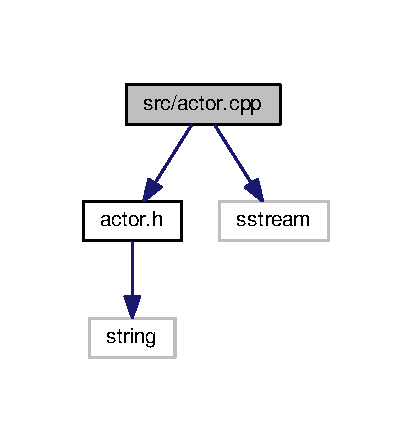
\includegraphics[width=198pt]{actor_8cpp__incl}
\end{center}
\end{figure}

\hypertarget{actor_8h}{}\section{src/actor.h File Reference}
\label{actor_8h}\index{src/actor.\+h@{src/actor.\+h}}
{\ttfamily \#include $<$string$>$}\\*
Include dependency graph for actor.\+h\+:
\nopagebreak
\begin{figure}[H]
\begin{center}
\leavevmode
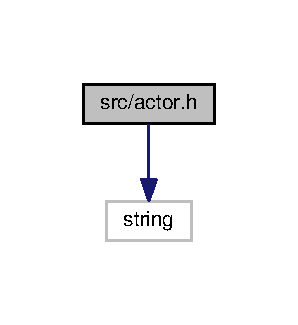
\includegraphics[width=143pt]{actor_8h__incl}
\end{center}
\end{figure}
This graph shows which files directly or indirectly include this file\+:
\nopagebreak
\begin{figure}[H]
\begin{center}
\leavevmode
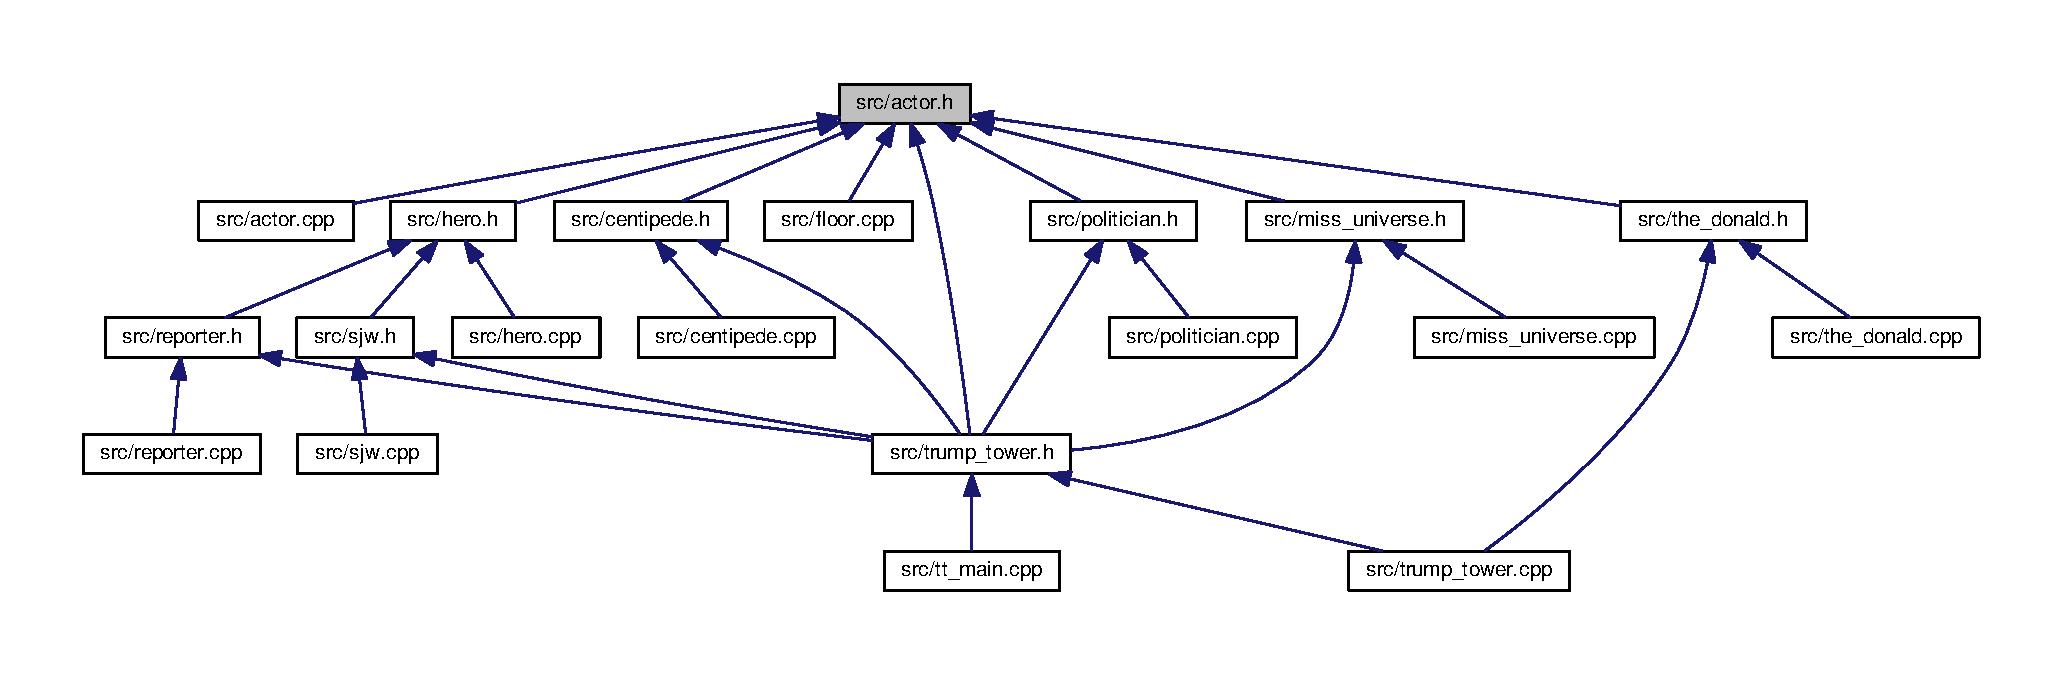
\includegraphics[width=350pt]{actor_8h__dep__incl}
\end{center}
\end{figure}
\subsection*{Classes}
\begin{DoxyCompactItemize}
\item 
class \hyperlink{classActor}{Actor}
\end{DoxyCompactItemize}

\hypertarget{centipede_8cpp}{}\section{src/centipede.cpp File Reference}
\label{centipede_8cpp}\index{src/centipede.\+cpp@{src/centipede.\+cpp}}
{\ttfamily \#include \char`\"{}centipede.\+h\char`\"{}}\\*
Include dependency graph for centipede.\+cpp\+:
\nopagebreak
\begin{figure}[H]
\begin{center}
\leavevmode
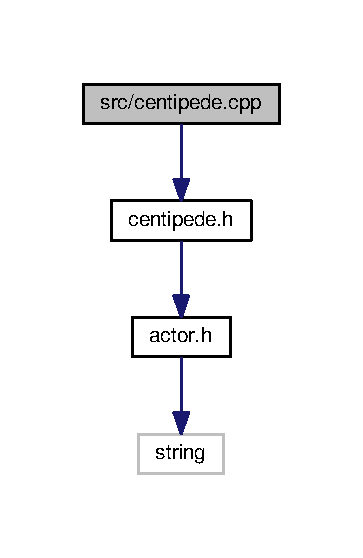
\includegraphics[width=174pt]{centipede_8cpp__incl}
\end{center}
\end{figure}

\hypertarget{centipede_8h}{}\section{src/centipede.h File Reference}
\label{centipede_8h}\index{src/centipede.\+h@{src/centipede.\+h}}
{\ttfamily \#include \char`\"{}actor.\+h\char`\"{}}\\*
Include dependency graph for centipede.\+h\+:
\nopagebreak
\begin{figure}[H]
\begin{center}
\leavevmode
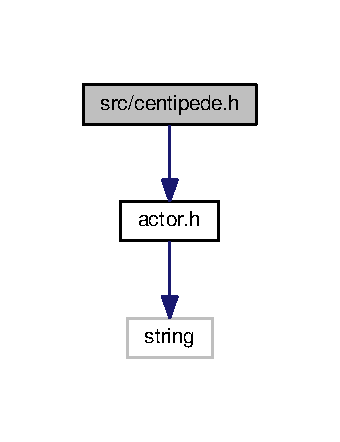
\includegraphics[width=163pt]{centipede_8h__incl}
\end{center}
\end{figure}
This graph shows which files directly or indirectly include this file\+:
\nopagebreak
\begin{figure}[H]
\begin{center}
\leavevmode
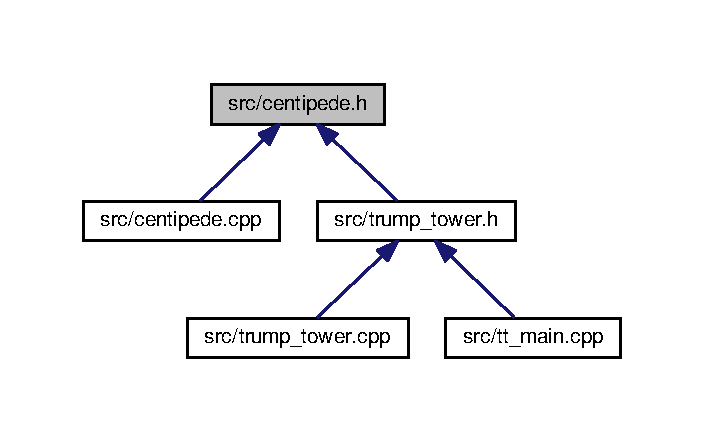
\includegraphics[width=338pt]{centipede_8h__dep__incl}
\end{center}
\end{figure}
\subsection*{Classes}
\begin{DoxyCompactItemize}
\item 
class \hyperlink{classCentipede}{Centipede}
\end{DoxyCompactItemize}

\hypertarget{direction_8h}{}\section{src/direction.h File Reference}
\label{direction_8h}\index{src/direction.\+h@{src/direction.\+h}}
{\ttfamily \#include $<$map$>$}\\*
{\ttfamily \#include $<$string$>$}\\*
Include dependency graph for direction.\+h\+:
\nopagebreak
\begin{figure}[H]
\begin{center}
\leavevmode
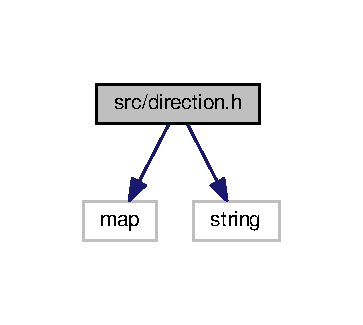
\includegraphics[width=174pt]{direction_8h__incl}
\end{center}
\end{figure}
This graph shows which files directly or indirectly include this file\+:
\nopagebreak
\begin{figure}[H]
\begin{center}
\leavevmode
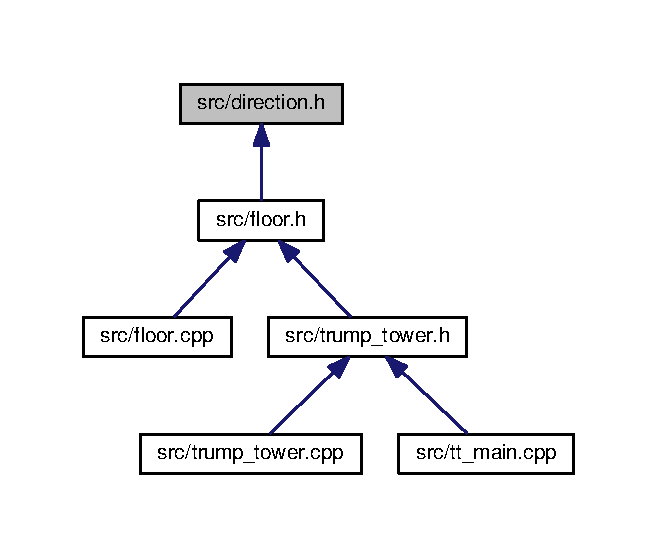
\includegraphics[width=316pt]{direction_8h__dep__incl}
\end{center}
\end{figure}
\subsection*{Enumerations}
\begin{DoxyCompactItemize}
\item 
enum \hyperlink{direction_8h_a224b9163917ac32fc95a60d8c1eec3aa}{Direction} \{ \hyperlink{direction_8h_a224b9163917ac32fc95a60d8c1eec3aaab5b3793b961949c817c7c0d99c05dad7}{E\+A\+ST}, 
\hyperlink{direction_8h_a224b9163917ac32fc95a60d8c1eec3aaae9449e8683a8199dad36b07a63b2f523}{W\+E\+ST}
 \}
\end{DoxyCompactItemize}


\subsection{Enumeration Type Documentation}
\index{direction.\+h@{direction.\+h}!Direction@{Direction}}
\index{Direction@{Direction}!direction.\+h@{direction.\+h}}
\subsubsection[{\texorpdfstring{Direction}{Direction}}]{\setlength{\rightskip}{0pt plus 5cm}enum {\bf Direction}}\hypertarget{direction_8h_a224b9163917ac32fc95a60d8c1eec3aa}{}\label{direction_8h_a224b9163917ac32fc95a60d8c1eec3aa}
\begin{Desc}
\item[Enumerator]\par
\begin{description}
\index{E\+A\+ST@{E\+A\+ST}!direction.\+h@{direction.\+h}}\index{direction.\+h@{direction.\+h}!E\+A\+ST@{E\+A\+ST}}\item[{\em 
E\+A\+ST\hypertarget{direction_8h_a224b9163917ac32fc95a60d8c1eec3aaab5b3793b961949c817c7c0d99c05dad7}{}\label{direction_8h_a224b9163917ac32fc95a60d8c1eec3aaab5b3793b961949c817c7c0d99c05dad7}
}]\index{W\+E\+ST@{W\+E\+ST}!direction.\+h@{direction.\+h}}\index{direction.\+h@{direction.\+h}!W\+E\+ST@{W\+E\+ST}}\item[{\em 
W\+E\+ST\hypertarget{direction_8h_a224b9163917ac32fc95a60d8c1eec3aaae9449e8683a8199dad36b07a63b2f523}{}\label{direction_8h_a224b9163917ac32fc95a60d8c1eec3aaae9449e8683a8199dad36b07a63b2f523}
}]\end{description}
\end{Desc}

\hypertarget{floor_8cpp}{}\section{src/floor.cpp File Reference}
\label{floor_8cpp}\index{src/floor.\+cpp@{src/floor.\+cpp}}
{\ttfamily \#include \char`\"{}floor.\+h\char`\"{}}\\*
{\ttfamily \#include $<$string$>$}\\*
{\ttfamily \#include \char`\"{}actor.\+h\char`\"{}}\\*
Include dependency graph for floor.\+cpp\+:
\nopagebreak
\begin{figure}[H]
\begin{center}
\leavevmode
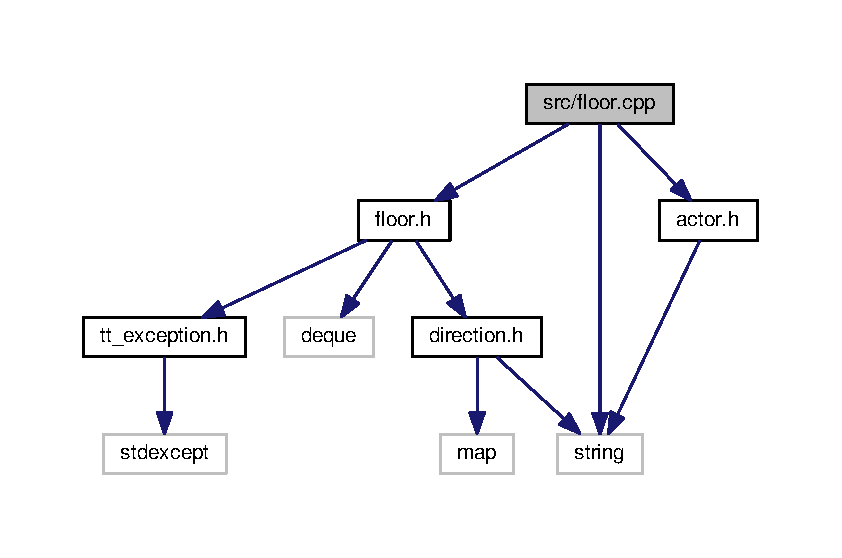
\includegraphics[width=350pt]{floor_8cpp__incl}
\end{center}
\end{figure}

\hypertarget{floor_8h}{}\section{src/floor.h File Reference}
\label{floor_8h}\index{src/floor.\+h@{src/floor.\+h}}
{\ttfamily \#include $<$deque$>$}\\*
{\ttfamily \#include \char`\"{}direction.\+h\char`\"{}}\\*
{\ttfamily \#include \char`\"{}tt\+\_\+exception.\+h\char`\"{}}\\*
Include dependency graph for floor.\+h\+:
\nopagebreak
\begin{figure}[H]
\begin{center}
\leavevmode
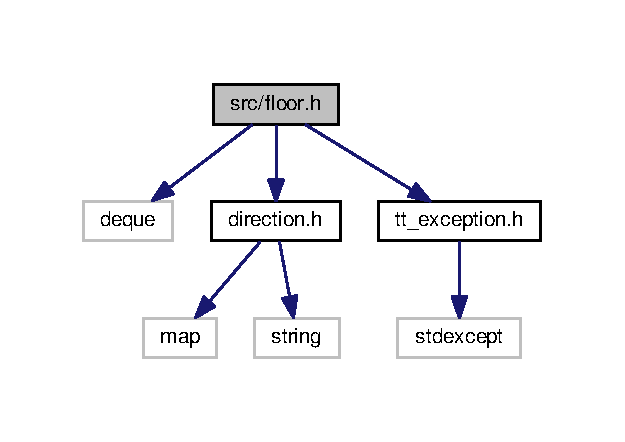
\includegraphics[width=300pt]{floor_8h__incl}
\end{center}
\end{figure}
This graph shows which files directly or indirectly include this file\+:
\nopagebreak
\begin{figure}[H]
\begin{center}
\leavevmode
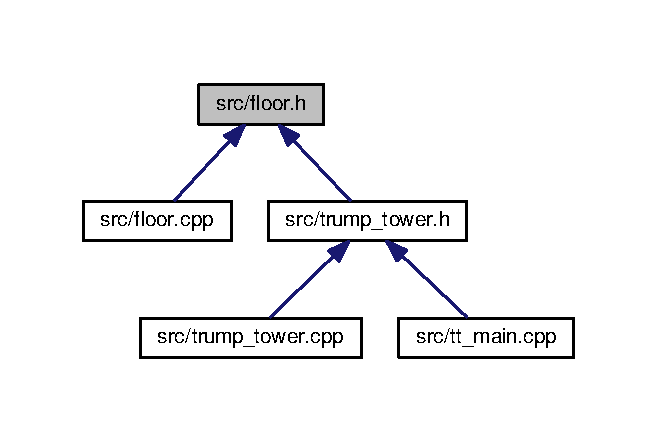
\includegraphics[width=316pt]{floor_8h__dep__incl}
\end{center}
\end{figure}
\subsection*{Classes}
\begin{DoxyCompactItemize}
\item 
class \hyperlink{classFloor}{Floor$<$ T $>$}
\end{DoxyCompactItemize}

\hypertarget{hero_8cpp}{}\section{src/hero.cpp File Reference}
\label{hero_8cpp}\index{src/hero.\+cpp@{src/hero.\+cpp}}
{\ttfamily \#include \char`\"{}hero.\+h\char`\"{}}\\*
{\ttfamily \#include \char`\"{}rng.\+h\char`\"{}}\\*
{\ttfamily \#include $<$iostream$>$}\\*
Include dependency graph for hero.\+cpp\+:
\nopagebreak
\begin{figure}[H]
\begin{center}
\leavevmode
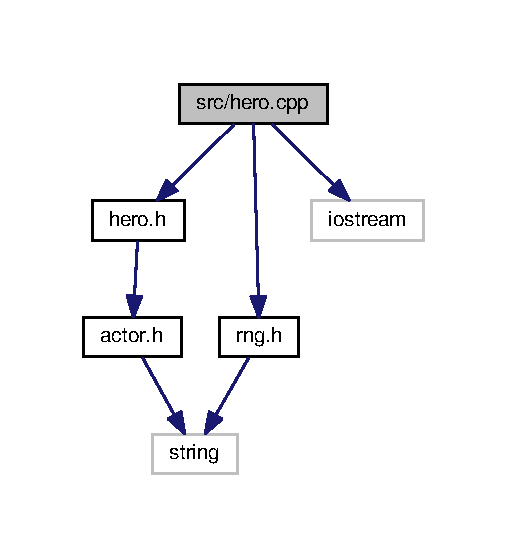
\includegraphics[width=244pt]{hero_8cpp__incl}
\end{center}
\end{figure}

\hypertarget{hero_8h}{}\section{src/hero.h File Reference}
\label{hero_8h}\index{src/hero.\+h@{src/hero.\+h}}
{\ttfamily \#include \char`\"{}actor.\+h\char`\"{}}\\*
Include dependency graph for hero.\+h\+:
\nopagebreak
\begin{figure}[H]
\begin{center}
\leavevmode
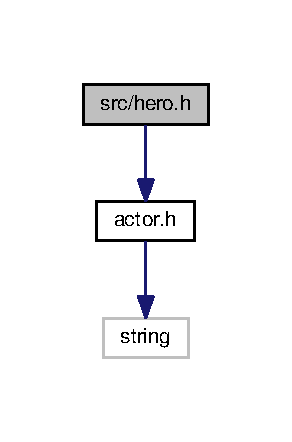
\includegraphics[width=140pt]{hero_8h__incl}
\end{center}
\end{figure}
This graph shows which files directly or indirectly include this file\+:
\nopagebreak
\begin{figure}[H]
\begin{center}
\leavevmode
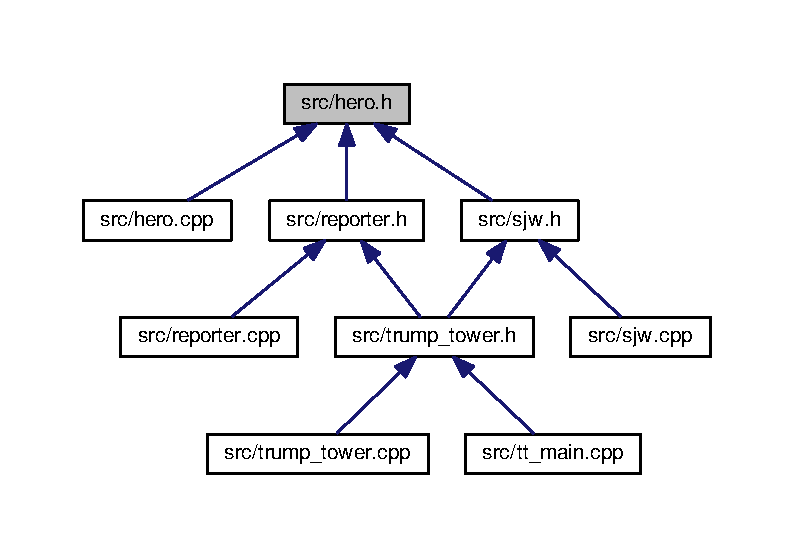
\includegraphics[width=350pt]{hero_8h__dep__incl}
\end{center}
\end{figure}
\subsection*{Classes}
\begin{DoxyCompactItemize}
\item 
class \hyperlink{classHero}{Hero}
\end{DoxyCompactItemize}

\hypertarget{log_8txt}{}\section{src/log.txt File Reference}
\label{log_8txt}\index{src/log.\+txt@{src/log.\+txt}}
\subsection*{Variables}
\begin{DoxyCompactItemize}
\item 
commit b927411a49611efa7be56566dfcf8370d925cf5e \hyperlink{log_8txt_a2153263aadf46404cd10eee1053d8cb2}{Author}
\end{DoxyCompactItemize}


\subsection{Variable Documentation}
\index{log.\+txt@{log.\+txt}!Author@{Author}}
\index{Author@{Author}!log.\+txt@{log.\+txt}}
\subsubsection[{\texorpdfstring{Author}{Author}}]{\setlength{\rightskip}{0pt plus 5cm}commit b927411a49611efa7be56566dfcf8370d925cf5e Author}\hypertarget{log_8txt_a2153263aadf46404cd10eee1053d8cb2}{}\label{log_8txt_a2153263aadf46404cd10eee1053d8cb2}

\hypertarget{miss__universe_8cpp}{}\section{src/miss\+\_\+universe.cpp File Reference}
\label{miss__universe_8cpp}\index{src/miss\+\_\+universe.\+cpp@{src/miss\+\_\+universe.\+cpp}}
{\ttfamily \#include \char`\"{}miss\+\_\+universe.\+h\char`\"{}}\\*
Include dependency graph for miss\+\_\+universe.\+cpp\+:
\nopagebreak
\begin{figure}[H]
\begin{center}
\leavevmode
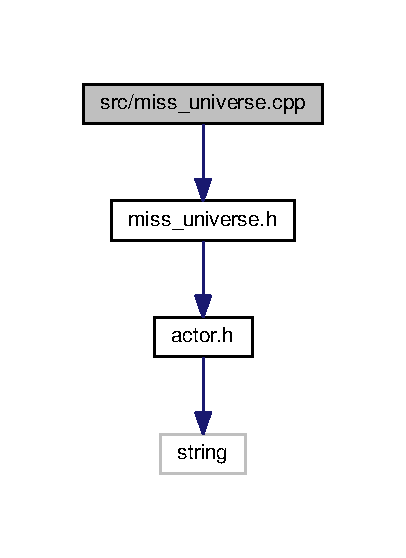
\includegraphics[width=195pt]{miss__universe_8cpp__incl}
\end{center}
\end{figure}

\hypertarget{miss__universe_8h}{}\section{src/miss\+\_\+universe.h File Reference}
\label{miss__universe_8h}\index{src/miss\+\_\+universe.\+h@{src/miss\+\_\+universe.\+h}}
{\ttfamily \#include \char`\"{}actor.\+h\char`\"{}}\\*
Include dependency graph for miss\+\_\+universe.\+h\+:
\nopagebreak
\begin{figure}[H]
\begin{center}
\leavevmode
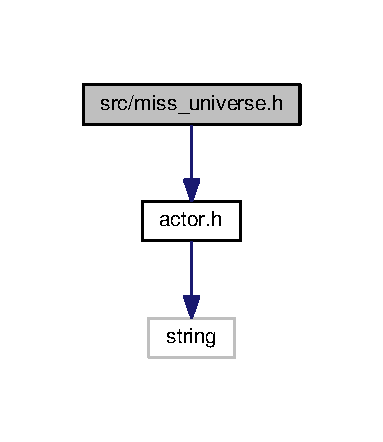
\includegraphics[width=184pt]{miss__universe_8h__incl}
\end{center}
\end{figure}
This graph shows which files directly or indirectly include this file\+:
\nopagebreak
\begin{figure}[H]
\begin{center}
\leavevmode
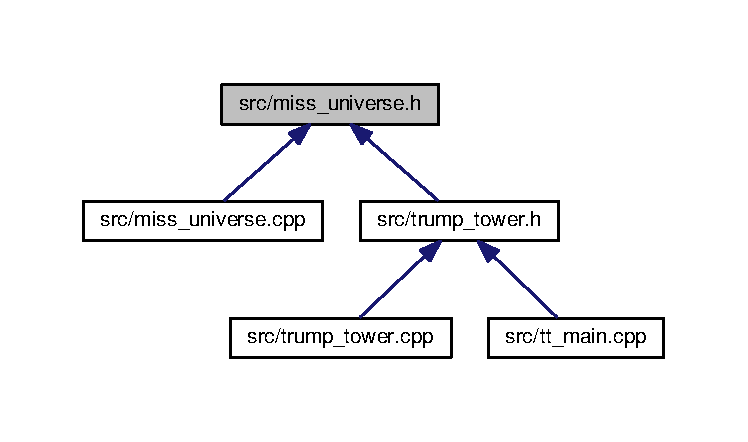
\includegraphics[width=350pt]{miss__universe_8h__dep__incl}
\end{center}
\end{figure}
\subsection*{Classes}
\begin{DoxyCompactItemize}
\item 
class \hyperlink{classMissUniverse}{Miss\+Universe}
\end{DoxyCompactItemize}

\hypertarget{politician_8cpp}{}\section{src/politician.cpp File Reference}
\label{politician_8cpp}\index{src/politician.\+cpp@{src/politician.\+cpp}}
{\ttfamily \#include \char`\"{}politician.\+h\char`\"{}}\\*
Include dependency graph for politician.\+cpp\+:
\nopagebreak
\begin{figure}[H]
\begin{center}
\leavevmode
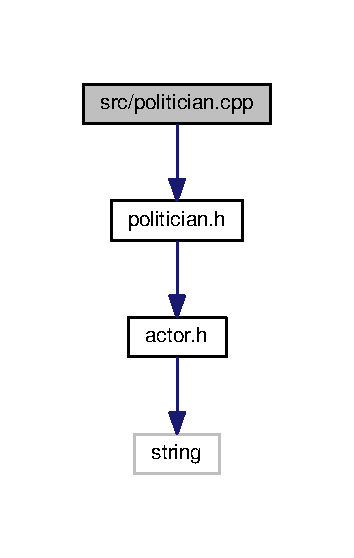
\includegraphics[width=170pt]{politician_8cpp__incl}
\end{center}
\end{figure}

\hypertarget{politician_8h}{}\section{src/politician.h File Reference}
\label{politician_8h}\index{src/politician.\+h@{src/politician.\+h}}
{\ttfamily \#include \char`\"{}actor.\+h\char`\"{}}\\*
Include dependency graph for politician.\+h\+:
\nopagebreak
\begin{figure}[H]
\begin{center}
\leavevmode
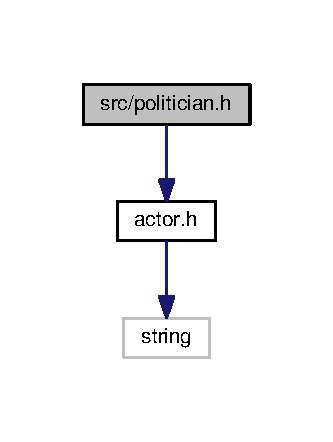
\includegraphics[width=160pt]{politician_8h__incl}
\end{center}
\end{figure}
This graph shows which files directly or indirectly include this file\+:
\nopagebreak
\begin{figure}[H]
\begin{center}
\leavevmode
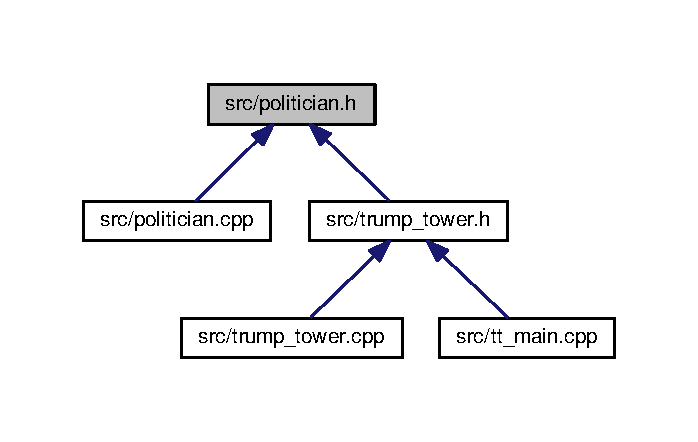
\includegraphics[width=335pt]{politician_8h__dep__incl}
\end{center}
\end{figure}
\subsection*{Classes}
\begin{DoxyCompactItemize}
\item 
class \hyperlink{classPolitician}{Politician}
\end{DoxyCompactItemize}

\hypertarget{rand__test_8cpp}{}\section{src/rand\+\_\+test.cpp File Reference}
\label{rand__test_8cpp}\index{src/rand\+\_\+test.\+cpp@{src/rand\+\_\+test.\+cpp}}
{\ttfamily \#include $<$cstdlib$>$}\\*
{\ttfamily \#include $<$iostream$>$}\\*
{\ttfamily \#include \char`\"{}rng.\+h\char`\"{}}\\*
Include dependency graph for rand\+\_\+test.\+cpp\+:
\nopagebreak
\begin{figure}[H]
\begin{center}
\leavevmode
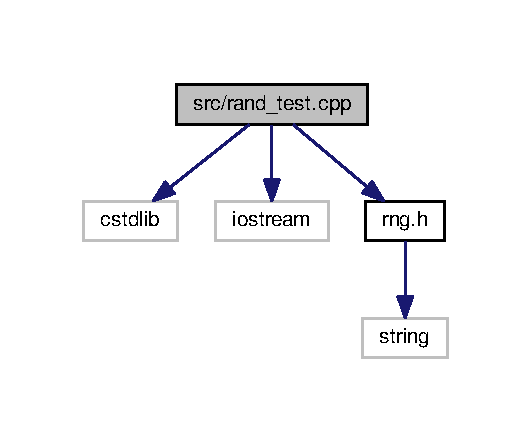
\includegraphics[width=255pt]{rand__test_8cpp__incl}
\end{center}
\end{figure}
\subsection*{Functions}
\begin{DoxyCompactItemize}
\item 
int \hyperlink{rand__test_8cpp_ae66f6b31b5ad750f1fe042a706a4e3d4}{main} ()
\end{DoxyCompactItemize}


\subsection{Function Documentation}
\index{rand\+\_\+test.\+cpp@{rand\+\_\+test.\+cpp}!main@{main}}
\index{main@{main}!rand\+\_\+test.\+cpp@{rand\+\_\+test.\+cpp}}
\subsubsection[{\texorpdfstring{main()}{main()}}]{\setlength{\rightskip}{0pt plus 5cm}int main (
\begin{DoxyParamCaption}
{}
\end{DoxyParamCaption}
)}\hypertarget{rand__test_8cpp_ae66f6b31b5ad750f1fe042a706a4e3d4}{}\label{rand__test_8cpp_ae66f6b31b5ad750f1fe042a706a4e3d4}
A test program for the random number generator.

\begin{DoxyReturn}{Returns}
E\+X\+I\+T\+\_\+\+S\+U\+C\+C\+E\+SS on completion 
\end{DoxyReturn}

\hypertarget{reporter_8cpp}{}\section{src/reporter.cpp File Reference}
\label{reporter_8cpp}\index{src/reporter.\+cpp@{src/reporter.\+cpp}}
{\ttfamily \#include \char`\"{}reporter.\+h\char`\"{}}\\*
Include dependency graph for reporter.\+cpp\+:
\nopagebreak
\begin{figure}[H]
\begin{center}
\leavevmode
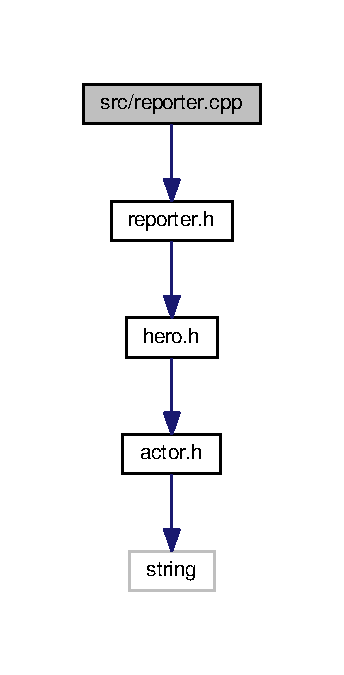
\includegraphics[width=165pt]{reporter_8cpp__incl}
\end{center}
\end{figure}

\hypertarget{reporter_8h}{}\section{src/reporter.h File Reference}
\label{reporter_8h}\index{src/reporter.\+h@{src/reporter.\+h}}
{\ttfamily \#include \char`\"{}hero.\+h\char`\"{}}\\*
Include dependency graph for reporter.\+h\+:
\nopagebreak
\begin{figure}[H]
\begin{center}
\leavevmode
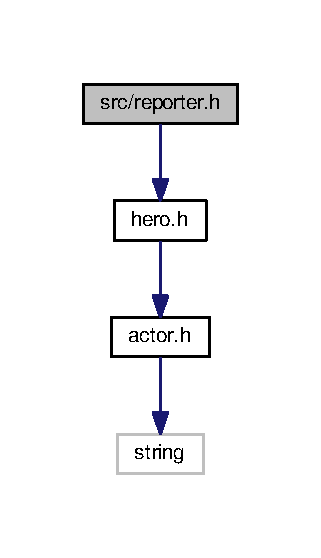
\includegraphics[width=154pt]{reporter_8h__incl}
\end{center}
\end{figure}
This graph shows which files directly or indirectly include this file\+:
\nopagebreak
\begin{figure}[H]
\begin{center}
\leavevmode
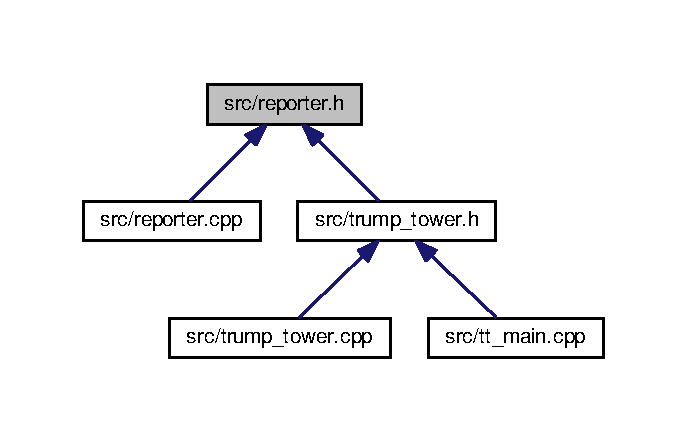
\includegraphics[width=330pt]{reporter_8h__dep__incl}
\end{center}
\end{figure}
\subsection*{Classes}
\begin{DoxyCompactItemize}
\item 
class \hyperlink{classReporter}{Reporter}
\end{DoxyCompactItemize}

\hypertarget{rng_8cpp}{}\section{src/rng.cpp File Reference}
\label{rng_8cpp}\index{src/rng.\+cpp@{src/rng.\+cpp}}
{\ttfamily \#include \char`\"{}rng.\+h\char`\"{}}\\*
{\ttfamily \#include $<$iostream$>$}\\*
Include dependency graph for rng.\+cpp\+:
\nopagebreak
\begin{figure}[H]
\begin{center}
\leavevmode
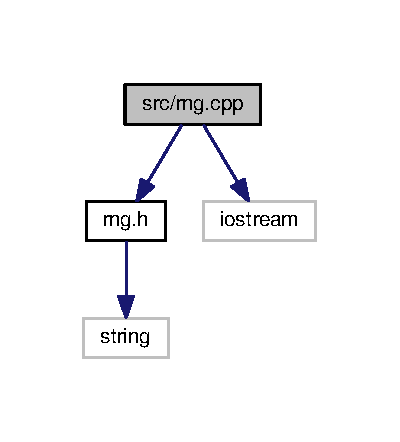
\includegraphics[width=192pt]{rng_8cpp__incl}
\end{center}
\end{figure}

\hypertarget{rng_8h}{}\section{src/rng.h File Reference}
\label{rng_8h}\index{src/rng.\+h@{src/rng.\+h}}
{\ttfamily \#include $<$string$>$}\\*
Include dependency graph for rng.\+h\+:
\nopagebreak
\begin{figure}[H]
\begin{center}
\leavevmode
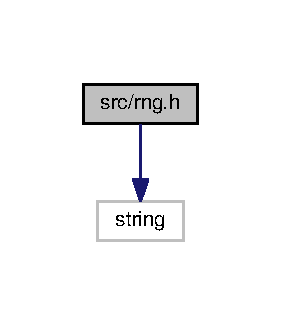
\includegraphics[width=135pt]{rng_8h__incl}
\end{center}
\end{figure}
This graph shows which files directly or indirectly include this file\+:
\nopagebreak
\begin{figure}[H]
\begin{center}
\leavevmode
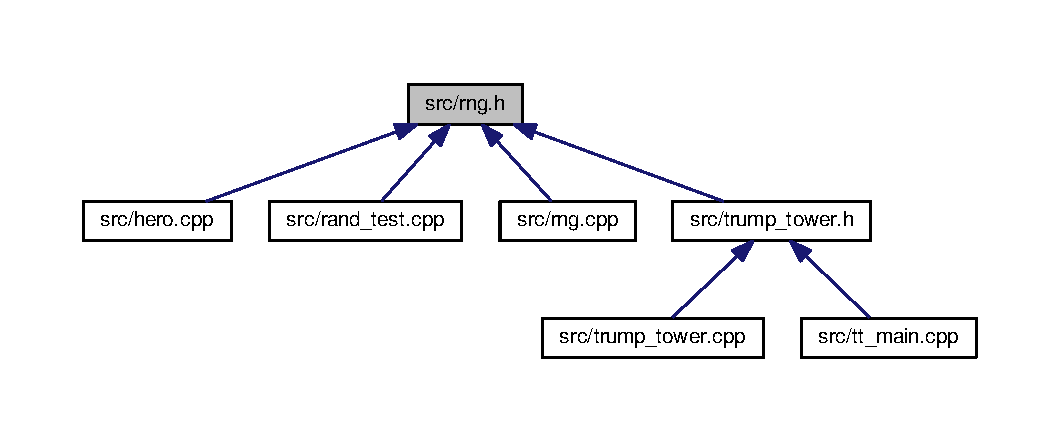
\includegraphics[width=350pt]{rng_8h__dep__incl}
\end{center}
\end{figure}
\subsection*{Classes}
\begin{DoxyCompactItemize}
\item 
class \hyperlink{classRNG}{R\+NG}
\end{DoxyCompactItemize}

\hypertarget{sjw_8cpp}{}\section{src/sjw.cpp File Reference}
\label{sjw_8cpp}\index{src/sjw.\+cpp@{src/sjw.\+cpp}}
{\ttfamily \#include \char`\"{}sjw.\+h\char`\"{}}\\*
Include dependency graph for sjw.\+cpp\+:
\nopagebreak
\begin{figure}[H]
\begin{center}
\leavevmode
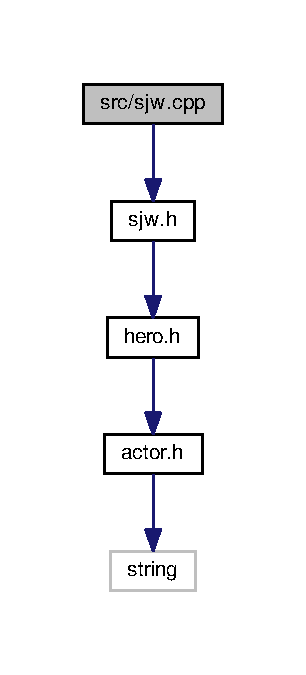
\includegraphics[width=147pt]{sjw_8cpp__incl}
\end{center}
\end{figure}

\hypertarget{sjw_8h}{}\section{src/sjw.h File Reference}
\label{sjw_8h}\index{src/sjw.\+h@{src/sjw.\+h}}
{\ttfamily \#include \char`\"{}hero.\+h\char`\"{}}\\*
Include dependency graph for sjw.\+h\+:
\nopagebreak
\begin{figure}[H]
\begin{center}
\leavevmode
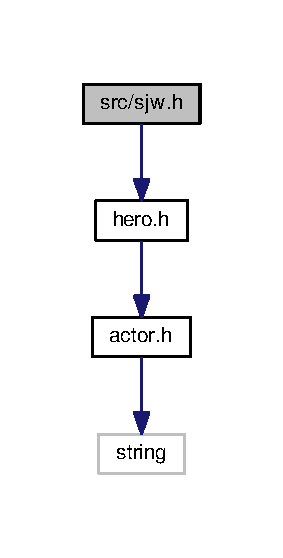
\includegraphics[width=136pt]{sjw_8h__incl}
\end{center}
\end{figure}
This graph shows which files directly or indirectly include this file\+:
\nopagebreak
\begin{figure}[H]
\begin{center}
\leavevmode
\includegraphics[width=312pt]{sjw_8h__dep__incl}
\end{center}
\end{figure}
\subsection*{Classes}
\begin{DoxyCompactItemize}
\item 
class \hyperlink{classSJW}{S\+JW}
\end{DoxyCompactItemize}

\hypertarget{the__donald_8cpp}{}\section{src/the\+\_\+donald.cpp File Reference}
\label{the__donald_8cpp}\index{src/the\+\_\+donald.\+cpp@{src/the\+\_\+donald.\+cpp}}
{\ttfamily \#include \char`\"{}the\+\_\+donald.\+h\char`\"{}}\\*
Include dependency graph for the\+\_\+donald.\+cpp\+:
\nopagebreak
\begin{figure}[H]
\begin{center}
\leavevmode
\includegraphics[width=179pt]{the__donald_8cpp__incl}
\end{center}
\end{figure}

\hypertarget{the__donald_8h}{}\section{src/the\+\_\+donald.h File Reference}
\label{the__donald_8h}\index{src/the\+\_\+donald.\+h@{src/the\+\_\+donald.\+h}}
{\ttfamily \#include \char`\"{}actor.\+h\char`\"{}}\\*
Include dependency graph for the\+\_\+donald.\+h\+:
\nopagebreak
\begin{figure}[H]
\begin{center}
\leavevmode
\includegraphics[width=169pt]{the__donald_8h__incl}
\end{center}
\end{figure}
This graph shows which files directly or indirectly include this file\+:
\nopagebreak
\begin{figure}[H]
\begin{center}
\leavevmode
\includegraphics[width=304pt]{the__donald_8h__dep__incl}
\end{center}
\end{figure}
\subsection*{Classes}
\begin{DoxyCompactItemize}
\item 
class \hyperlink{classTheDonald}{The\+Donald}
\end{DoxyCompactItemize}

\hypertarget{trump__tower_8cpp}{}\section{src/trump\+\_\+tower.cpp File Reference}
\label{trump__tower_8cpp}\index{src/trump\+\_\+tower.\+cpp@{src/trump\+\_\+tower.\+cpp}}
{\ttfamily \#include $<$cstdlib$>$}\\*
{\ttfamily \#include $<$iostream$>$}\\*
{\ttfamily \#include $<$string$>$}\\*
{\ttfamily \#include \char`\"{}trump\+\_\+tower.\+h\char`\"{}}\\*
{\ttfamily \#include \char`\"{}the\+\_\+donald.\+h\char`\"{}}\\*
Include dependency graph for trump\+\_\+tower.\+cpp\+:
\nopagebreak
\begin{figure}[H]
\begin{center}
\leavevmode
\includegraphics[width=350pt]{trump__tower_8cpp__incl}
\end{center}
\end{figure}

\hypertarget{trump__tower_8h}{}\section{src/trump\+\_\+tower.h File Reference}
\label{trump__tower_8h}\index{src/trump\+\_\+tower.\+h@{src/trump\+\_\+tower.\+h}}
{\ttfamily \#include $<$queue$>$}\\*
{\ttfamily \#include $<$set$>$}\\*
{\ttfamily \#include $<$stack$>$}\\*
{\ttfamily \#include $<$deque$>$}\\*
{\ttfamily \#include \char`\"{}actor.\+h\char`\"{}}\\*
{\ttfamily \#include \char`\"{}centipede.\+h\char`\"{}}\\*
{\ttfamily \#include \char`\"{}floor.\+h\char`\"{}}\\*
{\ttfamily \#include \char`\"{}miss\+\_\+universe.\+h\char`\"{}}\\*
{\ttfamily \#include \char`\"{}politician.\+h\char`\"{}}\\*
{\ttfamily \#include \char`\"{}reporter.\+h\char`\"{}}\\*
{\ttfamily \#include \char`\"{}rng.\+h\char`\"{}}\\*
{\ttfamily \#include \char`\"{}sjw.\+h\char`\"{}}\\*
Include dependency graph for trump\+\_\+tower.\+h\+:
\nopagebreak
\begin{figure}[H]
\begin{center}
\leavevmode
\includegraphics[width=350pt]{trump__tower_8h__incl}
\end{center}
\end{figure}
This graph shows which files directly or indirectly include this file\+:
\nopagebreak
\begin{figure}[H]
\begin{center}
\leavevmode
\includegraphics[width=288pt]{trump__tower_8h__dep__incl}
\end{center}
\end{figure}
\subsection*{Classes}
\begin{DoxyCompactItemize}
\item 
class \hyperlink{classTrumpTower}{Trump\+Tower}
\end{DoxyCompactItemize}

\hypertarget{tt__exception_8h}{}\section{src/tt\+\_\+exception.h File Reference}
\label{tt__exception_8h}\index{src/tt\+\_\+exception.\+h@{src/tt\+\_\+exception.\+h}}
{\ttfamily \#include $<$stdexcept$>$}\\*
Include dependency graph for tt\+\_\+exception.\+h\+:
\nopagebreak
\begin{figure}[H]
\begin{center}
\leavevmode
\includegraphics[width=175pt]{tt__exception_8h__incl}
\end{center}
\end{figure}
This graph shows which files directly or indirectly include this file\+:
\nopagebreak
\begin{figure}[H]
\begin{center}
\leavevmode
\includegraphics[width=316pt]{tt__exception_8h__dep__incl}
\end{center}
\end{figure}
\subsection*{Classes}
\begin{DoxyCompactItemize}
\item 
class \hyperlink{classTTException}{T\+T\+Exception}
\end{DoxyCompactItemize}

\hypertarget{tt__main_8cpp}{}\section{src/tt\+\_\+main.cpp File Reference}
\label{tt__main_8cpp}\index{src/tt\+\_\+main.\+cpp@{src/tt\+\_\+main.\+cpp}}
{\ttfamily \#include $<$cstdlib$>$}\\*
{\ttfamily \#include $<$iostream$>$}\\*
{\ttfamily \#include \char`\"{}trump\+\_\+tower.\+h\char`\"{}}\\*
Include dependency graph for tt\+\_\+main.\+cpp\+:
\nopagebreak
\begin{figure}[H]
\begin{center}
\leavevmode
\includegraphics[width=350pt]{tt__main_8cpp__incl}
\end{center}
\end{figure}
\subsection*{Functions}
\begin{DoxyCompactItemize}
\item 
int \hyperlink{tt__main_8cpp_a0ddf1224851353fc92bfbff6f499fa97}{main} (int argc, char $\ast$argv\mbox{[}$\,$\mbox{]})
\end{DoxyCompactItemize}


\subsection{Function Documentation}
\index{tt\+\_\+main.\+cpp@{tt\+\_\+main.\+cpp}!main@{main}}
\index{main@{main}!tt\+\_\+main.\+cpp@{tt\+\_\+main.\+cpp}}
\subsubsection[{\texorpdfstring{main(int argc, char $\ast$argv[])}{main(int argc, char *argv[])}}]{\setlength{\rightskip}{0pt plus 5cm}int main (
\begin{DoxyParamCaption}
\item[{int}]{argc, }
\item[{char $\ast$}]{argv\mbox{[}$\,$\mbox{]}}
\end{DoxyParamCaption}
)}\hypertarget{tt__main_8cpp_a0ddf1224851353fc92bfbff6f499fa97}{}\label{tt__main_8cpp_a0ddf1224851353fc92bfbff6f499fa97}
Program execution entry point 
\begin{DoxyParams}{Parameters}
{\em argc} & \+: number of arguments passed to the binary \\
\hline
{\em argv} & \+: argument passed to the binary \\
\hline
\end{DoxyParams}
\begin{DoxyReturn}{Returns}
0 if everything went well 
\end{DoxyReturn}

%--- End generated contents ---

% Index
\backmatter
\newpage
\phantomsection
\clearemptydoublepage
\addcontentsline{toc}{chapter}{Index}
\printindex

\end{document}
